\PassOptionsToPackage{svgnames,dvipsnames,svgnames}{xcolor}
\documentclass[sigplan,screen]{acmart}
\settopmatter{}
% \settopmatter{printfolios=true,printccs=true,printacmref=true}
%% For double-blind review submission, w/ CCS and ACM Reference
%\documentclass[acmsmall,review,anonymous]{acmart}\settopmatter{printfolios=true}
%% For single-blind review submission, w/o CCS and ACM Reference (max submission space)
%\documentclass[acmsmall,review]{acmart}\settopmatter{printfolios=true,printccs=false,printacmref=false}
%% For single-blind review submission, w/ CCS and ACM Reference
%\documentclass[acmsmall,review]{acmart}\settopmatter{printfolios=true}
%% For final camera-ready submission, w/ required CCS and ACM Reference
%\documentclass[acmsmall]{acmart}\settopmatter{}

%% Conference information
%% Supplied to authors by publisher for camera-ready submission;
%% use defaults for review submission.
% \acmConference[PL'21]{ACM SIGPLAN Conference on Programming Languages}{January 01--03, 2018}{New York, NY, USA}
% \acmYear{2021}
% \acmISBN{} % \acmISBN{978-x-xxxx-xxxx-x/YY/MM}
% \acmDOI{} % \acmDOI{10.1145/nnnnnnn.nnnnnnn}
% \startPage{1}
% \copyrightyear{2021}
% \acmYear{2021}
% \setcopyright{rightsretained}
% \acmConference[PLDI '21]{Proceedings of the 42nd ACM SIGPLAN International Conference on Programming Language Design and Implementation}{June 20--25, 2021}{Virtual Event, Canada}
% \acmBooktitle{Proceedings of the 42nd ACM SIGPLAN International Conference on Programming Language Design and Implementation (PLDI '21), June 20--25, 2021, Virtual Event, Canada}\acmDOI{10.1145/3453483.3454059}
% \acmISBN{978-1-4503-8391-2/21/06}
%% Copyright information
%% Supplied to authors (based on authors' rights management selection;
%% see authors.acm.org) by publisher for camera-ready submission;
%% use 'none' for review submission.
% \setcopyright{none}
%\setcopyright{acmcopyright}
%\setcopyright{acmlicensed}
%\setcopyright{rightsretained}
%\copyrightyear{2018}           %% If different from \acmYear

%% Bibliography style
% \bibliographystyle{ACM-Reference-Format}
%% Citation style
%\citestyle{acmauthoryear}  %% For author/year citations
%\citestyle{acmnumeric}     %% For numeric citations
%\setcitestyle{nosort}      %% With 'acmnumeric', to disable automatic
                            %% sorting of references within a single citation;
                            %% e.g., \cite{Smith99,Carpenter05,Baker12}
                            %% rendered as [14,5,2] rather than [2,5,14].
%\setcitesyle{nocompress}   %% With 'acmnumeric', to disable automatic
                            %% compression of sequential references within a
                            %% single citation;
                            %% e.g., \cite{Baker12,Baker14,Baker16}
                            %% rendered as [2,3,4] rather than [2-4].

%% Some recommended packages.
\usepackage{booktabs}   %% For formal tables:
                        %% http://ctan.org/pkg/booktabs
\usepackage{subcaption} %% For complex figures with subfigures/subcaptions
                        %% http://ctan.org/pkg/subcaption

%% Cyrus packages
\usepackage{microtype}
% \usepackage{mdframed}
% \usepackage{colortab}
\usepackage{mathpartir}
% \usepackage{enumitem}
% \usepackage{bbm}
\usepackage{stmaryrd}
% \usepackage{mathtools}
% \usepackage{leftidx}
\usepackage{todonotes}
\usepackage{xspace}
% \usepackage{wrapfig}
\usepackage{enumitem}
\usepackage{framed}
\usepackage{extarrows}

\usepackage{listings}%
\lstloadlanguages{ML}
\lstset{tabsize=2,
basicstyle=\footnotesize\ttfamily,
% keywordstyle=\sffamily,
commentstyle=\itshape\ttfamily\color{gray},
stringstyle=\ttfamily\color{purple},
mathescape=false,escapechar=\#,
numbers=left, numberstyle=\scriptsize\color{gray}\ttfamily, language=ML, showspaces=false,showstringspaces=false,xleftmargin=15pt,
morekeywords={string, float, int, Int, Float, String, livelit, at, SpliceRef, UpdateCmd, ViewCmd, Html, return,
context, Typ, Exp, Maybe, List, Result, Dim, Unit},
classoffset=0,belowskip=\smallskipamount, aboveskip=\smallskipamount,
xleftmargin=0cm,
moredelim=**[is][\color{red}]{SSTR}{ESTR}
}
\newcommand{\li}[1]{\lstinline[basicstyle=\ttfamily\fontsize{9pt}{1em}\selectfont]{#1}}
\newcommand{\lismall}[1]{\lstinline[basicstyle=\ttfamily\fontsize{9pt}{1em}\selectfont]{#1}}

%% Jana Dunfield macros
\def\OPTIONConf{1}%
\usepackage{janadunfield}

%% Can remove this eventually
% \usepackage{blindtext}

% \usepackage{enumitem}

%%%%%%%%%%%%%%%%%%%%%%%%%%%%%%%%%%%%%%%%%%%%%%%%%%%%%%%%%%%%%%%%%%%%%%%%%%%%%
%% Matt says: Cyrus, this package `adjustbox` seems directly related
%% to the `clipbox` error; To get rid of the error, I moved it last
%% (after other usepackages) and I added the line just above it, which
%% permits it to redefine `clipbox` (apparently also defined in
%% `pstricks`, and due to latex's complete lack of namespace
%% management, these would otherwise names clash).
% \let\clipbox\relax
% \usepackage[export]{adjustbox}% http://ctan.org/pkg/adjustbox
%%%%%%%%%%%%%%%%%%%%%%%%%%%%%%%%%%%%%%%%%%%%%%%%%%%%%%%%%%%%%%%%%%%%%%%%%%%%%%%%%


%%%%%%%%%%%%%%%%%%%%%%%%%%%%%%%%%%%%%%%%%%%%%%%%%%%%%%%%%%%%%%%%%%%%%%%%%%%%%%%%%
%\usepackage{draftwatermark}
%\SetWatermarkText{DRAFT}
%\SetWatermarkScale{1}
%%%%%%%%%%%%%%%%%%%%%%%%%%%%%%%%%%%%%%%%%%%%%%%%%%%%%%%%%%%%%%%%%%%%%%%%%%%%%%%%%


% \newtheorem{theorem}{Theorem}[chapter]
% \newtheorem{lemma}[theorem]{Lemma}
% \newtheorem{corollary}[theorem]{Corollary}
% \newtheorem{definition}[theorem]{Definition}
% \newtheorem{assumption}[theorem]{Assumption}
% \newtheorem{condition}[theorem]{Condition}

\newtheoremstyle{slplain}% name
  {.15\baselineskip\@plus.1\baselineskip\@minus.1\baselineskip}% Space above
  {.15\baselineskip\@plus.1\baselineskip\@minus.1\baselineskip}% Space below
  {\slshape}% Body font
  {\parindent}%Indent amount (empty = no indent, \parindent = para indent)
  {\bfseries}%  Thm head font
  {.}%       Punctuation after thm head
  { }%      Space after thm head: " " = normal interword space;
        %       \newline = linebreak
  {}%       Thm head spec
\theoremstyle{slplain}
\newtheorem{thm}{Theorem}  % Numbered with the equation counter
\numberwithin{thm}{section}
\newtheorem{defn}[thm]{Definition}
\newtheorem{lem}[thm]{Lemma}
\newtheorem{prop}[thm]{Proposition}
% \newtheorem{cor}[section]{Corollary}
% \newtheorem{lem}[section]{Lemma}
% \newtheorem{prop}[section]{Proposition}

% \setlength{\abovedisplayskip}{0pt}
% \setlength{\belowdisplayskip}{0pt}
% \setlength{\abovedisplayshortskip}{0pt}
% \setlength{\belowdisplayshortskip}{0pt}



\makeatletter\if@ACM@journal\makeatother
%% Journal information (used by PACMPL format)
%% Supplied to authors by publisher for camera-ready submission
% \acmJournal{PACMPL}
% \acmVolume{1}
% \acmNumber{1}
% \acmArticle{1}
% \acmYear{2018}
% \acmMonth{3}
% \acmDOI{10.1145/nnnnnnn.nnnnnnn}
\startPage{1}
\else\makeatother
%% Conference information (used by SIGPLAN proceedings format)
%% Supplied to authors by publisher for camera-ready submission
% \acmConference[]{ACM SIGPLAN Conference on Programming Languages}{January 01--03, 2017}{New York, NY, USA}

% \acmYear{2018}
% \acmISBN{978-x-xxxx-xxxx-x/YY/MM}
% \acmDOI{10.1145/nnnnnnn.nnnnnnn}
% \startPage{1}
\fi


%% Copyright information
%% Supplied to authors (based on authors' rights management selection;
%% see authors.acm.org) by publisher for camera-ready submission
% \setcopyright{none}             %% For review submission
%\setcopyright{acmcopyright}
%\setcopyright{acmlicensed}
%\setcopyright{rightsretained}
%\copyrightyear{2017}           %% If different from \acmYear


\fancyfoot{} % suppresses the footer (also need \thispagestyle{empty} after \maketitle below)


%% Bibliography style
\bibliographystyle{ACM-Reference-Format}
%% Citation style
%% Note: author/year citations are required for papers published as an
%% issue of PACMPL.
% \citestyle{acmauthoryear}   %% For author/year citations

% !TEX root = main.tex

\newcommand{\mynote}[3]{\textcolor{#3}{\textsf{{#2}}}}
\newcommand{\rkc}[1]{\mynote{rkc}{#1}{blue}}
\newcommand{\cy}[1]{\mynote{cy}{#1}{purple}}
\newcommand{\mah}[1]{\mynote{cy}{#1}{green}}
\newcommand{\matt}[1]{{\color{blue}{\textit{Matt:~#1}}}}

\newcommand{\cvert}{{\,{\vert}\,}}

%% https://tex.stackexchange.com/questions/9796/how-to-add-todo-notes
\newcommand{\rkcTodo}[1]{\todo[linecolor=blue,backgroundcolor=blue!25,bordercolor=blue]{#1}}

\newcommand{\mattTodo}[1]{\todo[linecolor=green,backgroundcolor=green!2,bordercolor=green]{\tiny\textit{#1}}}
\newcommand{\mattOmit}[1]{\colorbox{yellow}{(Matt omitted stuff here)}}

% \usepackage{amssymb}% http://ctan.org/pkg/amssymb
\usepackage{pifont}% http://ctan.org/pkg/pifont
\newcommand{\cmark}{\ding{51}}%
\newcommand{\xmark}{\ding{55}}%

\def\parahead#1{\paragraph{\textbf{#1.}}}
%% \def\paraheadNoDot#1{\paragraph{{\textbf{#1}}}}
\def\subparahead#1{\paragraph{\textit{#1.}}}
%% \def\paraheadindent#1{\paragraph{}\textit{#1.}}
%% \def\paraheadindentnodot#1{\paragraph{}\textit{#1}}

% \newcommand{\ie}{{\emph{i.e.}}}
% \newcommand{\eg}{{\emph{e.g.}}}
% \newcommand{\etc}{{\emph{etc.}}}
% \newcommand{\cf}{{\emph{cf.}}}
% \newcommand{\etal}{{\emph{et al.}}}

%% \newcommand{\hazel}{\ensuremath{\textsc{Hazel}}}
%% \newcommand{\sns}{\ensuremath{\textsc{Sketch-n-Sketch}}}
%% \newcommand{\deuce}{\ensuremath{\textsc{Deuce}}}
\newcommand{\Elm}{\ensuremath{\textsf{Elm}}}
\newcommand{\sns}
  %% {\ensuremath{\textrm{Sketch-n-Sketch}}}
  {\ensuremath{\textsf{Sketch-n-Sketch}}}
\newcommand{\deuce}
  %% {\ensuremath{\textrm{Deuce}}}
  {\ensuremath{\textsf{Deuce}}}

\newcommand{\sectionDescription}[1]{\section{#1}}
\newcommand{\subsectionDescription}[1]{\subsection{#1}}
\newcommand{\subsubsectionDescription}[1]{\subsubsection{#1}}
%% \newcommand{\subsectionDescription}[1]{\subsection*{#1}}
\newcommand{\suppMaterials}{the Supplementary Materials}

\newcommand{\defeq}{\overset{\textrm{def}}{=}}

\newcommand{\eap}{action suggestion panel\xspace}
\newcommand{\Eap}{Action suggestion panel\xspace}

\newcommand{\myfootnote}[1]{\footnote{ #1}}

\def\sectionautorefname{Section}
\def\subsectionautorefname{Section}
\def\subsubsectionautorefname{Section}

\newcommand{\code}[1]{\lstinline{#1}}

% Make italic?
%\newcommand{\Property}[1]{\emph{#1}}
\newcommand{\Property}[1]{\textrm{#1}}

% Calling out Cyrus's favorite verb, 'to be' ;)
\newcommand{\IS}{\colorbox{red}{is}\xspace}

\newcommand{\codeSize}
  %% {\footnotesize}
  {\small}

%\newcommand{\JoinTypes}[2]{\textsf{join}~~#1~~#2}
\newcommand{\JoinTypes}[2]{\textsf{join}(#1,#2)}

%%%%%%%%%%%%%%%%%%%%%%%%%%%%%%%%%%%%%%%%%%%%%%%%%%%%%%%%%%%%%%%%%%%%%%%%%%%%%%%%
%% Spacing

\newcommand{\sep}{\hspace{0.06in}}
\newcommand{\sepPremise}{\hspace{0.20in}}
\newcommand{\hsepRule}{\hspace{0.20in}}
\newcommand{\vsepRuleHeight}{0.08in}
\newcommand{\vsepRule}{\vspace{\vsepRuleHeight}}
\newcommand{\miniSepOne}{\hspace{0.01in}}
\newcommand{\miniSepTwo}{\hspace{0.02in}}
\newcommand{\miniSepThree}{\hspace{0.03in}}
\newcommand{\miniSepFour}{\hspace{0.04in}}
\newcommand{\miniSepFive}{\hspace{0.05in}}

%%%%%%%%%%%%%%%%%%%%%%%%%%%%%%%%%%%%%%%%%%%%%%%%%%%%%%%%%%%%%%%%%%%%%%%%%%%%%%%%

% \lstset{
% %mathescape=true,basicstyle=\fontsize{8}{9}\ttfamily,
% literate={=>}{$\Rightarrow$}2
%          {<=}{$\leq$}2
%          {->}{${\rightarrow}$}1
%          {\\\\=}{\color{red}{$\lambda$}}2
%          {\\\\}{$\lambda$}2
%          {**}{$\times$}2
%          {*.}{${\color{blue}{\texttt{*.}}}$}2
%          {+.}{${\color{blue}{\texttt{+.}}}$}2
%          {<}{${\color{green}{\lhd}}$}1
%          {>?}{${\color{green}{\rhd}}$?}2
%          {<<}{${\color{green}{\blacktriangleleft}}$}1
%          {>>?}{${\color{green}{\blacktriangleright}}$?}2
%          {\{}{${\color{blue}{\{}}$}1
%          {\}}{${\color{blue}{\}}}$}1
%          {[}{${\color{purple}{[}}$}1
%          {]}{${\color{purple}{]}}$}1
%          {(}{${\color{darkgray}{\texttt{(}}}$}1
%          {)}{${\color{darkgray}{\texttt{)}}}$}1
%          {]]}{${\color{gray}{\big(}}$}1
%          {]]}{${\color{gray}{\big)}}$}1
% }

% !TEX root = prelim-paper.tex

% \newcommand{\Label}[1]{\vspace{-20px}\label{#1}%
%   {\small\textcolor{cyan}{(\texttt{#1})}}\vspace{20px}%
% }

\newcommand{\note}[1]{\textcolor{blue}{#1}}
\newcommand{\tylr}{\texttt{tylr}}
\newcommand{\ty}{\textsf{tylrcore}}

% Violet hot dog buns; highlight color helps distinguish them
\newcommand{\llparenthesiscolor}{\textcolor{violet}{\llparenthesis}}
\newcommand{\rrparenthesiscolor}{\textcolor{violet}{\rrparenthesis}}

\newcommand{\styp}{t}
\newcommand{\spat}{p}
\newcommand{\sexp}{e}
\newcommand{\shole}{\llparenthesiscolor\rrparenthesiscolor}
\newcommand{\svar}[1]{#1}
\newcommand{\snum}{\texttt{num}}
\newcommand{\sbool}{\texttt{bool}}
\newcommand{\sarr}[2]{#1 \rightarrow #2}
\newcommand{\tprod}{\texttt{,}}
\newcommand{\sprod}[2]{#1\texttt{,}#2}
\newcommand{\sann}[2]{#1~\texttt{:}~#2}
\newcommand{\sboollit}[1]{#1}
\newcommand{\snumlit}[1]{#1}
\newcommand{\sparen}[1]{\texttt{(}#1\texttt{)}}
\newcommand{\tlam}[1]{\lambda #1.}
\newcommand{\slam}[2]{\lambda #1.#2}
\newcommand{\tlet}[2]{\texttt{let}~#1~\texttt{=}~#2~\texttt{in}}
\newcommand{\slet}[3]{\texttt{let}~#1~\texttt{=}~#2~\texttt{in}~#3}
\newcommand{\tplus}{\texttt{+}}
\newcommand{\splus}[2]{#1~\tplus~#2}
\newcommand{\tmult}{\texttt{*}}
\newcommand{\smult}[2]{#1~\texttt{*}~#2}
\newcommand{\tdiv}{\texttt{/}}
\newcommand{\sdiv}[2]{#1~\texttt{/}~#2}
\newcommand{\sequals}[2]{#1~\texttt{==}~#2}
\newcommand{\sap}[2]{#1\texttt{\textvisiblespace}#2}
\newcommand{\scond}[3]{#1~\texttt{?}~#2~\texttt{:}~#3}

\newcommand{\sbinhole}[2]{#1~\binhole~#2}

\newcommand{\action}{a}
\newcommand{\actionlit}[1]{\texttt{#1}}
\newcommand{\direction}{d}

\newcommand{\ophole}{%

\begin{tikzpicture}%
\draw[line width=0.75pt,gray]
  (-0.25ex,0.5ex)
  -- (0,1ex)
  -- (0.5ex,1ex)
  -- (0.75ex,0.5ex)
  -- (0.5ex,0)
  -- (0,0)
  -- cycle;%
\end{tikzpicture}%
}
\newcommand{\binhole}{%

\begin{tikzpicture}%
\draw[line width=0.65pt,gray]
  (0,0.5ex)
  -- (-0.25ex,1ex)
  -- (0.75ex,1ex)
  -- (0.5ex,0.5ex)
  -- (0.75ex,0)
  -- (-0.25ex,0)
  -- cycle;%
\end{tikzpicture}%
}

% \newcommand{\optile}[1]{\mbox{$\langle\overline{\underline{\text{#1\vphantom{|}}}}\rangle$}}
% \newcommand{\pretile}[1]{\mbox{$\langle\overline{\underline{\text{#1\vphantom{|}}}}\langle$}}
% \newcommand{\posttile}[1]{\mbox{$\rangle\overline{\underline{\text{#1\vphantom{|}}}}\rangle$}}
% \newcommand{\bintile}[1]{\mbox{$\rangle\overline{\underline{\text{#1\vphantom{|}}}}\langle$}}

\newcommand{\ltiletip}{{\color{gray}\langle}}
\newcommand{\rtiletip}{{\color{gray}\rangle}}

\newcommand{\toptile}[1]{\mbox{$\ltiletip\text{#1\vphantom{|}}\rtiletip$}}
\newcommand{\tpretile}[1]{\mbox{$\ltiletip\text{#1\vphantom{|}}\ltiletip$}}
\newcommand{\tposttile}[1]{\mbox{$\rtiletip\text{#1\vphantom{|}}\rtiletip$}}
\newcommand{\tbintile}[1]{\mbox{$\rtiletip\text{#1\vphantom{|}}\ltiletip$}}

\newcommand{\optile}[1]{\mbox{$\ltiletip\text{$#1$\vphantom{|}}\rtiletip$}}
\newcommand{\pretile}[1]{\mbox{$\ltiletip\text{$#1$\vphantom{|}}\ltiletip$}}
\newcommand{\posttile}[1]{\mbox{$\rtiletip\text{$#1$\vphantom{|}}\rtiletip$}}
\newcommand{\bintile}[1]{\mbox{$\rtiletip\text{$#1$\vphantom{|}}\ltiletip$}}


\newcommand{\tterm}[1]{\toptile{#1}}
\newcommand{\term}[1]{\optile{#1}}

\newcommand{\editState}{Z}
\newcommand{\performAction}[3]{#1 \xlongrightarrow{#2} #3}
\newcommand{\pmove}[3]{#1 \xlongrightarrow{\actionlit{move}~#2}_{\texttt{p}} #3}
\newcommand{\smove}[3]{#1 \xlongrightarrow{\actionlit{move}~#2}_{\texttt{s}} #3}
\newcommand{\rmove}[3]{#1 \xlongrightarrow{\actionlit{move}~#2}_{\texttt{r}} #3}

\newcommand{\tiles}{T}
\newcommand{\tile}{t}
\newcommand{\shard}{h}
\newcommand{\shardlit}[1]{\underline{#1}}
\newcommand{\selection}{C}
\newcommand{\selem}{c}
\newcommand{\tframe}{F}
\newcommand{\tfrelem}{f}
% \newcommand{\tframelit}[2]{#1 ~\gg~ #2}
\newcommand{\tframelit}[2]{#1\ \ \rotatebox[origin=c]{90}{\textcolor{black!35!}{$\boldsymbol\gg$}}\ \ #2}

\newcommand{\zip}{Z}
\newcommand{\zipper}[2]{#1\ \rotatebox[origin=c]{90}{\textcolor{black!40!}{$\boldsymbol\gtrdot$}}\ #2}
\newcommand{\subject}{B}
\newcommand{\zframe}{M}
\newcommand{\pointing}[2]{#1\hspace{-3pt}\multimapbothvert\hspace{-3pt}#2}
\newcommand{\selecting}[3]{#1\hspace{-3pt}\multimapbothvert\hspace{-3pt}\overline{#2}#3}
\newcommand{\restructuring}[3]{#1\hspace{-3pt}\multimapbothvert\hspace{-3pt}\widehat{#2}#3}

\newcommand{\leftTip}[1]{\overleftarrow{#1}}
\newcommand{\rightTip}[1]{\overrightarrow{#1}}
\newcommand{\ltip}{\langle}
\newcommand{\rtip}{\rangle}
\newcommand{\fixHolesEnd}[3]{#1\rightsquigarrow_{#2}#3}
\newcommand{\fixHoles}[4]{\pointing{#1}{#2}\rightsquigarrow\pointing{#3}{#4}}
\newcommand{\fixHolesFn}[2]{fixHoles(#1, #2)}

\newcommand{\leftSort}[1]{\overleftarrow{#1}^s}
\newcommand{\rightSort}[1]{\overrightarrow{#1}^s}

\newcommand{\lltip}[1]{\setlength\fboxsep{2pt}\colorbox{black!10!}{$\langle^{#1}$}}
\newcommand{\rrtip}[1]{\setlength\fboxsep{2pt}\colorbox{black!10!}{$\rangle^{#1}$}}
\newcommand{\tip}{\tau}
\newcommand{\sortoftip}[1]{\mathsf{sort}\left(#1\right)}

\newcommand{\lTip}{lt}
\newcommand{\rTip}{rt}
\newcommand{\ltipconv}[1]{{}^{#1}\langle}
\newcommand{\ltipconc}[1]{{}^{#1}\rangle}
\newcommand{\rtipconv}[1]{\rangle^{#1}}
\newcommand{\rtipconc}[1]{\langle^{#1}}

\newcommand{\matchesSort}[2]{#1~\texttt{matchesSort}~#2}
\newcommand{\fits}[2]{#1~\texttt{fits}~#2}

\newcommand{\wholeSelection}[2]{\texttt{whole}_{#1}~#2}

\newcommand{\filterTiles}[2]{\mathsf{filterTiles}_{#1}(#2)}

% \newcommand{\fixholes}[4]{#1~#2~#3\rightsquigarrow#4}

\newcommand{\ishole}[1]{#1~\mathsf{hole}}

\newcommand{\fixHolesSelection}[4]{#1~#2\rightsquigarrow#3~#4}
\newcommand{\fixHolesSelections}[4]{#1\mid#2\rightsquigarrow#3\mid#4}

\newcommand{\parseSelection}[1]{\left\lceil#1\right\rceil}
\newcommand{\parseZipper}[1]{\left\lfloor#1\right\rfloor}

\newcommand{\typ}{\texttt{typ}}
\newcommand{\pat}{\texttt{pat}}
\newcommand{\expr}{\texttt{exp}}

% \newcommand{\tpiecedd}{\scalebox{1.2}{\rotatebox[origin=c]{-45}{$\twoheadrightarrow$}}}
\newcommand{\tpiecedd}{\Searrow}
\newcommand{\pieceDisassembles}[2]{#1\tpiecedd#2}

\newcommand{\tpiecesdd}{\searrow}

\newcommand{\tframedu}{\Nearrow}
\newcommand{\framedu}[2]{#1 \tframedu #2}
\newcommand{\tzipperdu}{\nearrow}
\newcommand{\zipperdu}[2]{#1 \tzipperdu #2}

\newcommand{\disassemblesDown}[2]{#1 \searrow #2}
\newcommand{\disassemblesUp}[2]{#1 \nearrow #2}

\newcommand{\disassembleTile}[1]{\left\lfloor~#1~\right\rfloor}
\newcommand{\disassembleTileFrame}[1]{\left\lceil~#1~\right\rceil}

\newcommand{\stepDisassembleSelection}[2]{#1 \searrow #2}
\newcommand{\disassembleSelection}[2]{#1 \succeq #2}
\newcommand{\disassembleZipper}[2]{#1 \nearrow #2}

\newcommand{\flattenTerm}[2]{#1\hookrightarrow#2}

\newcommand{\cmttclo}[2]{\mathsf{clo}(#1, #2)}

% \newcommand{\CaptionLabel}[2]{
%   \caption{#1 {\small\textcolor{cyan}{(#2)}}}
%   \label{#2}}
\newcommand{\CaptionLabel}[2]{
  \caption{#1}
  \label{#2}}

% \newcommand{\llparenthesiscolor}{\textcolor{red}{\lfloor}}
% \newcommand{\rrparenthesiscolor}{\textcolor{red}{\rfloor}}

\newcommand{\fmap} [3] {\{ #1 ~ \rotatebox[origin=c]{180}{$\Lsh$} ~ #3 \}_{#1 \in #2}}

%% TODO if feeling really obsessive, use the following in place of x,u,c,b
\newcommand{\varVar}{x}
\newcommand{\varHole}{u}
\newcommand{\econst}{c}
\newcommand{\tbase}{b}

% HTyp and HExp
\newcommand{\isComplete}[1]{#1~\mathsf{complete}}

\newcommand{\tconsistent}[2]{#1 \sim #2}
\newcommand{\tinconsistent}[2]{#1 \nsim #2}
\newcommand{\tconsistentc}[2]{#1 \sim_c #2}

% Expression forms
\newcommand{\hexp}{e} % Hexp without palettes
\newcommand{\pexp}{p} % Meta variable for palette expressions
\newcommand{\encExp}{\mathtt{Exp}} % Whatever htyp encoded things should have

% HExp
\newcommand{\hlam}[2]{\lambda #1.#2}
\newcommand{\halam}[3]{\lambda #1{:}#2.#3}
\newcommand{\hap}[2]{#1~#2}
\newcommand{\hapP}[2]{(#1)~(#2)} % Extra paren around function term
\newcommand{\hpair}[2]{(#1, #2)}
\newcommand{\hprj}[2]{\mathsf{prj}_{#1}(#2)}
\newcommand{\hprl}[1]{\mathsf{prl}(#1)}
\newcommand{\hprr}[1]{\mathsf{prr}(#1)}
\newcommand{\htriv}{()}
\newcommand{\lblL}{\mathsf{L}}
\newcommand{\lblR}{\mathsf{R}}
\newcommand{\hnum}[1]{\underline{#1}}
\newcommand{\helet}[3]{\mathsf{let}~#1=#2~\mathsf{in}~#3}
%\newcommand{\hcase}[5]{\mathsf{case}\,#1\,\mathsf{of}\,#2\Rightarrow#3~\vert~#4\Rightarrow#5}
\newcommand{\hadd}[2]{#1 + #2}
\newcommand{\hehole}[1]{\llparenthesiscolor\rrparenthesiscolor^{#1}}
% \newcommand{\hhole}[1]{\setlength{\fboxsep}{0pt}\fcolorbox{red}{white}{\vphantom{)}$#1$}}
\newcommand{\hhole}[2]{\llparenthesiscolor#1\rrparenthesiscolor^{#2}}
% \newcommand{\hhole}[1]{
  % \setlength{\fboxsep}{0pt}
  % \colorbox{violet!10!white!100}{\ensuremath{\llparenthesiscolor#1\rrparenthesiscolor}}}
\newcommand{\hindet}[1]{\lceil#1\rceil}
%\newcommand{\hinj}[2]{\texttt{inj}_{#1}({#2})}
\newcommand{\hinL}[1]{\mathsf{inl}(#1)}
\newcommand{\hinR}[1]{\mathsf{inr}(#1)}
\newcommand{\hcase}[5]{\texttt{case}({#1},{#2}.{#3},{#4}.{#5})}
\newcommand{\hroll}[1]{\mathsf{roll}(#1)}
\newcommand{\hunroll}[1]{\mathsf{unroll}(#1)}
\newcommand{\livelitname}[1]{\$#1}
\newcommand{\haplivelit}[4]{\livelitname{#2}\langle #3; #4 \rangle^{#1}}
\newcommand{\hsplice}[2]{#1 : #2}

% Palettes
\newcommand{\pexpPalLet}[3]{\keyword{let palette}\,#1\,\keyword{=}\,#2\,\keyword{in}\,#3}
\newcommand{\pexpPalAp}[4]{#1 \left(#2;\,#4 : #3 \right)}
\newcommand{\pexpPalApF}[3]{#1 \left(#2;\,#3\right)}

% Palette definitions
\newcommand{\pDef}{\pi} % Meta variable for palette definitions
\newcommand{\pDefRecord}[3]{\{ \mathsf{expand}: #1, \, \mathsf{modelTyp}: #2, \, \mathsf{expandTyp}: #3\}}
\newcommand{\pDefRecordF}[4]{\{ \mathsf{expand}: #1, \, \mathsf{modelTyp}: #2, \, \mathsf{spliceTyp}: #3, \, \mathsf{expandTyp}: #4\}}
\newcommand{\pPhiWF}[1]{#1 \, \, \mathsf{palctx}}

\newcommand{\hGamma}{\Gamma}
\newcommand{\pPhi}{\Phi}
\newcommand{\EmptyhGamma}{\emptyset}
\newcommand{\EmptyDelta}{\emptyset}
\newcommand{\domof}[1]{\text{dom}(#1)}
\newcommand{\hsyn}[3]{#1 \vdash #2 \Rightarrow #3}
\newcommand{\hana}[3]{#1 \vdash #2 \Leftarrow #3}

% ZTyp and ZExp
\newcommand{\zlsel}[1]{{\bowtie}{#1}}
\newcommand{\zrsel}[1]{{#1}{\bowtie}}

%\newcommand{\zwsel}[1]{\adjustbox{cframe=blue}{\ensuremath{{\textcolor{blue}{\triangleright}}{#1}{\textcolor{blue}{\triangleleft}}}}}
\newcommand{\zwsel}[1]{
  \setlength{\fboxsep}{0pt}
  \colorbox{green!10!white!100}{
    \ensuremath{{{\textcolor{Green}{{\hspace{-2px}\triangleright}}}}{#1}{\textcolor{Green}{\triangleleft{\vphantom{\tehole}}}}}}
}
%\newcommand{\zwsel}[1]{{\triangleright}{#1}{\triangleleft}}

\newcommand{\removeSel}[1]{#1^{\diamond}}

% ZTyp
\newcommand{\ztau}{\hat{\tau}}

% ZExp
\newcommand{\zexp}{\hat{e}}

% Direction
\newcommand{\dParent}{\mathtt{parent}}
\newcommand{\dChild}{\mathtt{firstChild}}
\newcommand{\dNext}{\mathtt{nextSib}}
\newcommand{\dPrev}{\mathtt{prevSib}}

% Action
\newcommand{\aMove}[1]{\mathtt{move}~#1}
	\newcommand{\zrightmost}[1]{\mathsf{rightmost}(#1)}
	\newcommand{\zleftmost}[1]{\mathsf{leftmost}(#1)}
\newcommand{\aSelect}[1]{\mathtt{sel}~#1}
\newcommand{\aDel}{\mathtt{del}}
\newcommand{\aReplace}[1]{\mathtt{replace}~#1}
\newcommand{\aConstruct}[1]{\mathtt{construct}~#1}
\newcommand{\aConstructx}[1]{#1}
\newcommand{\aFinish}{\mathtt{finish}}

\newcommand{\performAna}[5]{#1 \vdash #2 \xlongrightarrow{#4} #5 \Leftarrow #3}
\newcommand{\performAnaI}[5]{#1 \vdash #2 \xlongrightarrow{#4}\hspace{-3px}{}^{*}~ #5 \Leftarrow #3}
\newcommand{\performSyn}[6]{#1 \vdash #2 \Rightarrow #3 \xlongrightarrow{#4} #5 \Rightarrow #6}
\newcommand{\performSynI}[6]{#1 \vdash #2 \Rightarrow #3 \xlongrightarrow{#4}\hspace{-3px}{}^{*}~ #5 \Rightarrow #6}
\newcommand{\performTyp}[3]{#1 \xlongrightarrow{#2} #3}
\newcommand{\performTypI}[3]{#1 \xlongrightarrow{#2}\hspace{-3px}{}^{*}~#3}

\newcommand{\performMove}[3]{#1 \xlongrightarrow{#2} #3}
\newcommand{\performDel}[2]{#1 \xlongrightarrow{\aDel} #2}

% Form
\newcommand{\farr}{\mathtt{arrow}}
\newcommand{\fnum}{\mathtt{num}}
\newcommand{\fsum}{\mathtt{sum}}

\newcommand{\fasc}{\mathtt{asc}}
\newcommand{\fvar}[1]{\mathtt{var}~#1}
\newcommand{\flam}[1]{\mathtt{lam}~#1}
\newcommand{\fap}{\mathtt{ap}}
\newcommand{\farg}{\mathtt{arg}}
\newcommand{\fnumlit}[1]{\mathtt{lit}~#1}
\newcommand{\fplus}{\mathtt{plus}}
\newcommand{\fhole}{\mathtt{hole}}
\newcommand{\fnehole}{\mathtt{nehole}}

\newcommand{\finj}[1]{\mathtt{inj}~#1}
\newcommand{\fcase}[2]{\mathtt{case}~#1~#2}

% Talk about formal rules in example
\newcommand{\refrule}[1]{\textrm{Rule~(#1)}}

\newcommand{\herase}[1]{\left|#1\right|_\textsf{erase}}

\newcommand{\arrmatch}[2]{#1 \blacktriangleright_{\rightarrow} #2}
%% TODO maybe write underbracket
%% \newcommand{\groundmatch}[2]{\underline{#1} = #2}
\newcommand{\groundmatch}[2]{#1 \blacktriangleright_{\mathsf{ground}} #2}
\newcommand{\prodmatch}[2]{#1 \blacktriangleright_{\times} #2}
\newcommand{\summatch}[2]{#1 \blacktriangleright_{+} #2}


\newcommand{\TABperformAna}[5]{#1 \vdash & #2                & \xlongrightarrow{#4} & #5 & \Leftarrow #3}
\newcommand{\TABperformSyn}[6]{#1 \vdash & #2 \Rightarrow #3 & \xlongrightarrow{#4} & #5 \Rightarrow #6}
\newcommand{\TABperformTyp}[3]{& #1 & \xlongrightarrow{#2} & #3}

\newcommand{\TABperformMove}[3]{#1 & \xlongrightarrow{#2} & #3}
\newcommand{\TABperformDel}[2]{#1 \xlongrightarrow{\aDel} #2}

\newcommand{\sumhasmatched}[2]{#1 \mathrel{\textcolor{black}{\blacktriangleright_{+}}} #2}

%%%% DYNAMICS %%%%
%% TODO remove these macros
%% marks for eval
\newcommand{\unevaled}{\times}
\newcommand{\evaled}{\checkmark}
\newcommand{\markname}{m}

\newcommand{\mvar}[0]{u}
\newcommand{\subst}[0]{\sigma}
\newcommand{\substitute}[3]{[#1/#2]#3}
\newcommand{\substitutesub}[4]{[#1/#2]_{#3}\,#4}
\newcommand{\fvof}[1]{\mathsf{FV}(#1)}
\newcommand{\dexp}[0]{d}
\newcommand{\dconst}[0]{c}
\newcommand{\dval}[0]{\ddot{v}}
%% TODO remove this macro
\newcommand{\dcast}[2]{\langle #1 \rangle ~ #2}
%% TODO make the following two look better
\newcommand{\dcasttwo}[3]{#1 \langle{#2}\Rightarrow{#3}\rangle}
\newcommand{\dcastthree}[4]
  {#1 \langle{#2}\Rightarrow{#3}\Rightarrow{#4}\rangle} %% sugared version
  %% {\dcasttwo{\dcasttwo{#1}{#2}{#3}}{#3}{#4}} %% unsugared version
\newcommand{\dcastfail}[3]{#1 \langle{#2}\Rightarrow{\tehole}\not\Rightarrow{#3}\rangle}
%% \newcommand{\dlam}[3]{\lambda #1:#2.#3}
\newcommand{\dlam}[3]{\halam{#1}{#2}{#3}}
\newcommand{\dap}[2]{#1(#2)}
\newcommand{\dapP}[2]{(#1)(#2)} % Extra paren around function term
\newcommand{\dnum}[1]{\underline{#1}}
%\newcommand{\dcase}[5]{\mathsf{case}\,#1\,\mathsf{of}\,#2\Rightarrow#3~\vert~#4\Rightarrow#5}
\newcommand{\dadd}[2]{#1 + #2}
%% TODO third arg should be empty
\newcommand{\dehole}[2]{{\llparenthesiscolor\rrparenthesiscolor}{^{#1}_{#2}}}
%% TODO fourth arg should be empty
\newcommand{\dhole}[4]{\leftidx{^{#4}}{\llparenthesiscolor#1\rrparenthesiscolor}{^{#2}_{#3}}}
\newcommand{\dindet}[1]{\lceil#1\rceil}
%\newcommand{\dinj}[2]{\texttt{inj}_{#1}({#2})}
\newcommand{\dinL}[2]{\mathsf{inl}_{#1}(#2)}
\newcommand{\dinR}[2]{\mathsf{inr}_{#1}(#2)}
\newcommand{\dcase}[5]{\texttt{case}({#1},{#2}.{#3},{#4}.{#5})}
\newcommand{\dpair}[2]{(#1,#2)}
\newcommand{\dprj}[2]{\mathsf{prj}_{#1}(#2)}

\newcommand{\isType}[2]{#1 \vdash #2~\mathtt{type}}
\newcommand{\elabs}[5]{#1 \vdash #2 \leadsto #3 : #4 \dashv #5}
\newcommand{\expands}[5]{#1; #2 \vdash #3 \leadsto #4 : #5}
\newcommand{\ccexpands}[6]{#1; #2 \vdash_\text{cc} #3 \leadsto #4 : #5 \dashv #6}
\newcommand{\Omegaitem}[2]{#1 \hookrightarrow #2}
\newcommand{\expandAna}[6]{#1 \vdash #2 \Leftarrow #3 \leadsto #4 : #5 \dashv #6}
\newcommand{\expandSyn}[5]{#1 \vdash #2 \Rightarrow #3 \leadsto #4 \dashv #5}
\newcommand{\pexpandAna}[5]{#1 \vdash_{#2} #3 \leadsto #4 \Leftarrow #5}
\newcommand{\pexpandSyn}[5]{#1 \vdash_{#2} #3 \leadsto #4 \Rightarrow #5}
\newcommand{\decodeExp}[2]{#1 \uparrow #2}
\newcommand{\encodeExp}[2]{#1 \downarrow #2}
\newcommand{\hasType}[3]{#1 \vdash #2 : #3}
\newcommand{\hasTypeD}[4]{#1; #2 \vdash #3 : #4}
\newcommand{\isValue}[1]{#1~\mathsf{val}}
\newcommand{\isGround}[1]{#1~\mathsf{ground}}
\newcommand{\isBoxedValue}[1]{#1~\mathsf{boxedval}}
\newcommand{\isIndet}[1]{#1~\mathsf{indet}}
\newcommand{\isFinal}[1]{#1~\mathsf{final}}
\newcommand{\isErr}[2]{#1 \vdash #2~\mathsf{err}}
%% \newcommand{\stepsTo}[2]{#1 \mapsto_{\Delta} #2}
%% TODO first arg should be empty
%% \newcommand{\stepsToD}[3]{#1 \vdash #2 \mapsto #3}
\newcommand{\stepsToD}[3]{#2 \mapsto #3}
\newcommand{\multiStepsTo}[2]{#1 \mapsto^* #2}
\newcommand{\evalsTo}[2]{#1 \Downarrow #2}

%% TODO if feeling obsessive, replace direct uses of \Delta
\newcommand{\hDelta}{\Delta}
\newcommand{\Dunion}[2]{#1 \cup #2}
\newcommand{\idof}[1]{\mathsf{id}(#1)}
\newcommand{\Dbinding}[3]{#1 :: #3[#2]}
\newcommand{\instantiate}[3]{\llbracket#1 / #2\rrbracket #3}
\newcommand{\instantiateB}[2]{\llbracket #1 / #2\rrbracket}

% Contextual dynamics
\newcommand{\evalctx}{\mathcal{E}}
\newcommand{\evalhole}{\circ}
\newcommand{\isevalctx}[1]{#1~\mathsf{evalCtx}}
%% TODO first arg should be empty
%% \newcommand{\reducesE}[3]{#1 \vdash #2 \longrightarrow #3}
\newcommand{\reducesE}[3]{#2 \longrightarrow #3}
\newcommand{\selectEvalCtxR}[2]{#1\{#2\}}
\newcommand{\selectEvalCtx}[3]{#1=\selectEvalCtxR{#2}{#3}}
\newcommand{\maybePremise}[1]{{\textcolor{red}[}#1{\textcolor{red}]}}

\newcommand{\inhole}[2]{\mathsf{inhole}(#1; #2)}

\newcommand{\DoSubst}[3]{[#1/#2]{#3}}

\newcommand{\splat}[1]{\{#1\}_{i < n}}
\newcommand{\taut}[1]{\tau_\text{#1}}
\newcommand{\etxt}[1]{e_\text{#1}}
\newcommand{\dtxt}[1]{d_\text{#1}}
\newcommand{\splices}{\splat{\psi_i}}

\newcommand{\livelitCtxEntry}[4]{\mathsf{livelit}~\livelitname{#1}~\mathsf{at}~#2~\{#3; #4\}}
\newcommand{\expType}{\mathsf{Exp}}
\newcommand{\livelitsIn}[1]{\mathsf{livelits}(#1)}
\newcommand{\protoEnvsOf}[3]{\mathsf{protoenvs}_{#1}(#2; #3)}
\newcommand{\envsOf}[3]{\mathsf{envs}_{#1}(#2; #3)}
\newcommand{\fillof}[2]{\mathsf{fill}_{#1}(#2)}
\newcommand{\resumeof}[1]{\mathsf{resume}(#1)}


\setlength{\abovecaptionskip}{4pt plus 6pt minus 6pt} % Chosen fairly arbitrarily
\setlength{\belowcaptionskip}{-4pt plus 6pt minus 6pt} % Chosen fairly arbitrarily


\begin{document}

%% Title information
\title
  [Linear Structure Editing]
  {Linear Structure Editing}
  %% [Programming by Direct Manipulation of Palettes]
  %% {Functional Programming by\\Direct Manipulation of Live Palette Expressions}

                                        %% when present, will be used in
                                        %% header instead of Full Title.
% \titlenote{with title note}             %% \titlenote is optional;
                                        %% can be repeated if necessary;
                                        %% contents suppressed with 'anonymous'
% \subtitle{Subtitle}                     %% \subtitle is optional
% \subtitlenote{with subtitle note}       %% \subtitlenote is optional;
                                        %% can be repeated if necessary;
                                        %% contents suppressed with 'anonymous'


%% Author information
%% Contents and number of authors suppressed with 'anonymous'.
%% Each author should be introduced by \author, followed by
%% \authornote (optional), \orcid (optional), \affiliation, and
%% \email.
%% An author may have multiple affiliations and/or emails; repeat the
%% appropriate command.
%% Many elements are not rendered, but should be provided for metadata
%% extraction tools.

%% Author with single affiliation.
\author{David Moon}
% \authornote{with author1 note}          %% \authornote is optional;
                                        %% can be repeated if necessary
% \orcid{nnnn-nnnn-nnnn-nnnn}             %% \orcid is optional
\affiliation{
  % \position{Position1}
  % \department{Department1}              %% \department is recommended
  \institution{University of Michigan}            %% \institution is required
  % \streetaddress{Street1 Address1}
  \city{Ann Arbor}
  \state{MI}
  % \postcode{Post-Code1}
  \country{USA}
}
\email{dmoo@umich.edu}          %% \email is recommended

\author{Cyrus Omar}
% \authornote{with author1 note}          %% \authornote is optional;
                                        %% can be repeated if necessary
% \orcid{nnnn-nnnn-nnnn-nnnn}             %% \orcid is optional
\affiliation{
  % \position{Position1}
  % \department{Department1}              %% \department is recommended
  \institution{University of Michigan}            %% \institution is required
  % \streetaddress{Street1 Address1}
  \city{Ann Arbor}
  \state{MI}
  % \postcode{Post-Code1}
  \country{USA}
}
\email{comar@umich.edu}          %% \email is recommended

% %% Author with two affiliations and emails.
% \author{First2 Last2}
% \authornote{with author2 note}          %% \authornote is optional;
%                                         %% can be repeated if necessary
% \orcid{nnnn-nnnn-nnnn-nnnn}             %% \orcid is optional
% \affiliation{
%   \position{Position2a}
%   \department{Department2a}             %% \department is recommended
%   \institution{Institution2a}           %% \institution is required
%   \streetaddress{Street2a Address2a}
%   \city{City2a}
%   \state{State2a}
%   \postcode{Post-Code2a}
%   \country{Country2a}
% }
% \email{first2.last2@inst2a.com}         %% \email is recommended
% \affiliation{
%   \position{Position2b}
%   \department{Department2b}             %% \department is recommended
%   \institution{Institution2b}           %% \institution is required
%   \streetaddress{Street3b Address2b}
%   \city{City2b}
%   \state{State2b}
%   \postcode{Post-Code2b}
%   \country{Country2b}
% }
% \email{first2.last2@inst2b.org}         %% \email is recommended


%% Paper note
%% The \thanks command may be used to create a "paper note" ---
%% similar to a title note or an author note, but not explicitly
%% associated with a particular element.  It will appear immediately
%% above the permission/copyright statement.
% \thanks{with paper note}                %% \thanks is optional
                                        %% can be repeated if necesary
                                        %% contents suppressed with 'anonymous'


%% Abstract
%% Note: \begin{abstract}...\end{abstract} environment must come
%% before \maketitle command
% !TEX root = prelim-paper.tex

\begin{abstract}
  Structure editors have long promised to improve the programming experience for all,
  but are often too slow or difficult to use.
  We describe a new approach to structure editing, called tile-based editing,
  that recovers many of the flexible and linear editing affordances of text editors.
  We describe \tylr~, a tiny tile-based editor;
  sketch the beginnings of a formal calculus called \ty~ that precisely specifies
  the mechanics and guarantees of tile-based editing;
  and describe our ongoing work to scale up tile-based editing
  to support larger program authoring.
\end{abstract}



%% 2012 ACM Computing Classification System (CSS) concepts
%% Generate at 'http://dl.acm.org/ccs/ccs.cfm'.
% \begin{CCSXML}
% <ccs2012>
% <concept>
% <concept_id>10011007.10011006.10011008</concept_id>
% <concept_desc>Software and its engineering~General programming languages</concept_desc>
% <concept_significance>500</concept_significance>
% </concept>
% <concept>
% <concept_id>10003456.10003457.10003521.10003525</concept_id>
% <concept_desc>Social and professional topics~History of programming languages</concept_desc>
% <concept_significance>300</concept_significance>
% </concept>
% </ccs2012>
% \end{CCSXML}

% \ccsdesc[500]{Software and its engineering~General programming languages}
% \ccsdesc[300]{Social and professional topics~History of programming languages}
%% End of generated code


%% Keywords
%% comma separated list
% \keywords{keyword1, keyword2, keyword3}  %% \keywords is optional
\keywords{structure editing}


%% \maketitle
%% Note: \maketitle command must come after title commands, author
%% commands, abstract environment, Computing Classification System
%% environment and commands, and keywords command.
\maketitle
% \thispagestyle{empty} % suppresses the footer

\section{Introduction}\label{sec:intro}

\emph{Structure editors}
have long promised to improve the programming experience
for beginners and experts alike.
By eliminating parse errors,
they provide cognitive benefits for novices
  \cite{meta-analysis-blocks,blocks-text-high-school,coblox}
  and end-users
  \cite{weitnauer2016graspable,rousillon,BasHermans21};
  simplify language composition
  \cite{mbeddr}
  and language-aware editor tooling
  \cite{HazelnutSNAPL};
  and form an essential component of truly continuous live programming
  \cite{Hazelnut,HazelnutLive}.
Yet, in the forty years since the idea was first
introduced and implemented \cite{Cornell},
structure editing has failed to reach
mainstream use by programmers beyond the novice level.
The problem, as many have observed
\cite{user-modeling,fine-tuning-selection-semantics,
practical-lang-based-editing,lang-on-the-usefulness,
psg,Minor92,TowardUserFriendly,MillerPMV94},
is that structure editors can be too slow
or difficult to use.

For example, while
block-based editors like Scratch \cite{scratch}
excel at introducing programming
to children and end-users, they soon become unwieldy
as users gain experience and create larger programs.
Cited issues include their inefficient mouse-driven
input, low visual information density, and rigid
tree-based construction of operator sequences
\cite{BlocksFingertips,cog-dim-blocks,blocks-and-beyond,no-keyboard-cripples}.

Meanwhile, the JetBrains MPS \cite{DBLP:conf/icse/VoelterP12}
editor resolves those particular issues with
keyboard-driven text-like interfaces---and
is used regularly by some professional programmers---but
instead suffers from steep learning curves and difficult-to-predict
editing behavior.
Consider the violin plots in Figure \ref{fig:mps-violin-plots},
which show post-task questionnaire responses from
a controlled user study of MPS \cite{ProjEfficiency}.
The left two plots show that MPS novices felt that
selection was relatively slow and inaccurate despite
a 45-minute training session and another 30-45 minutes
worth of study tasks.
Meanwhile, the right two plots show that
MPS novices and \emph{experts} alike struggled to
predict the effects of deletion.

\begin{figure}[b]
  \centering
  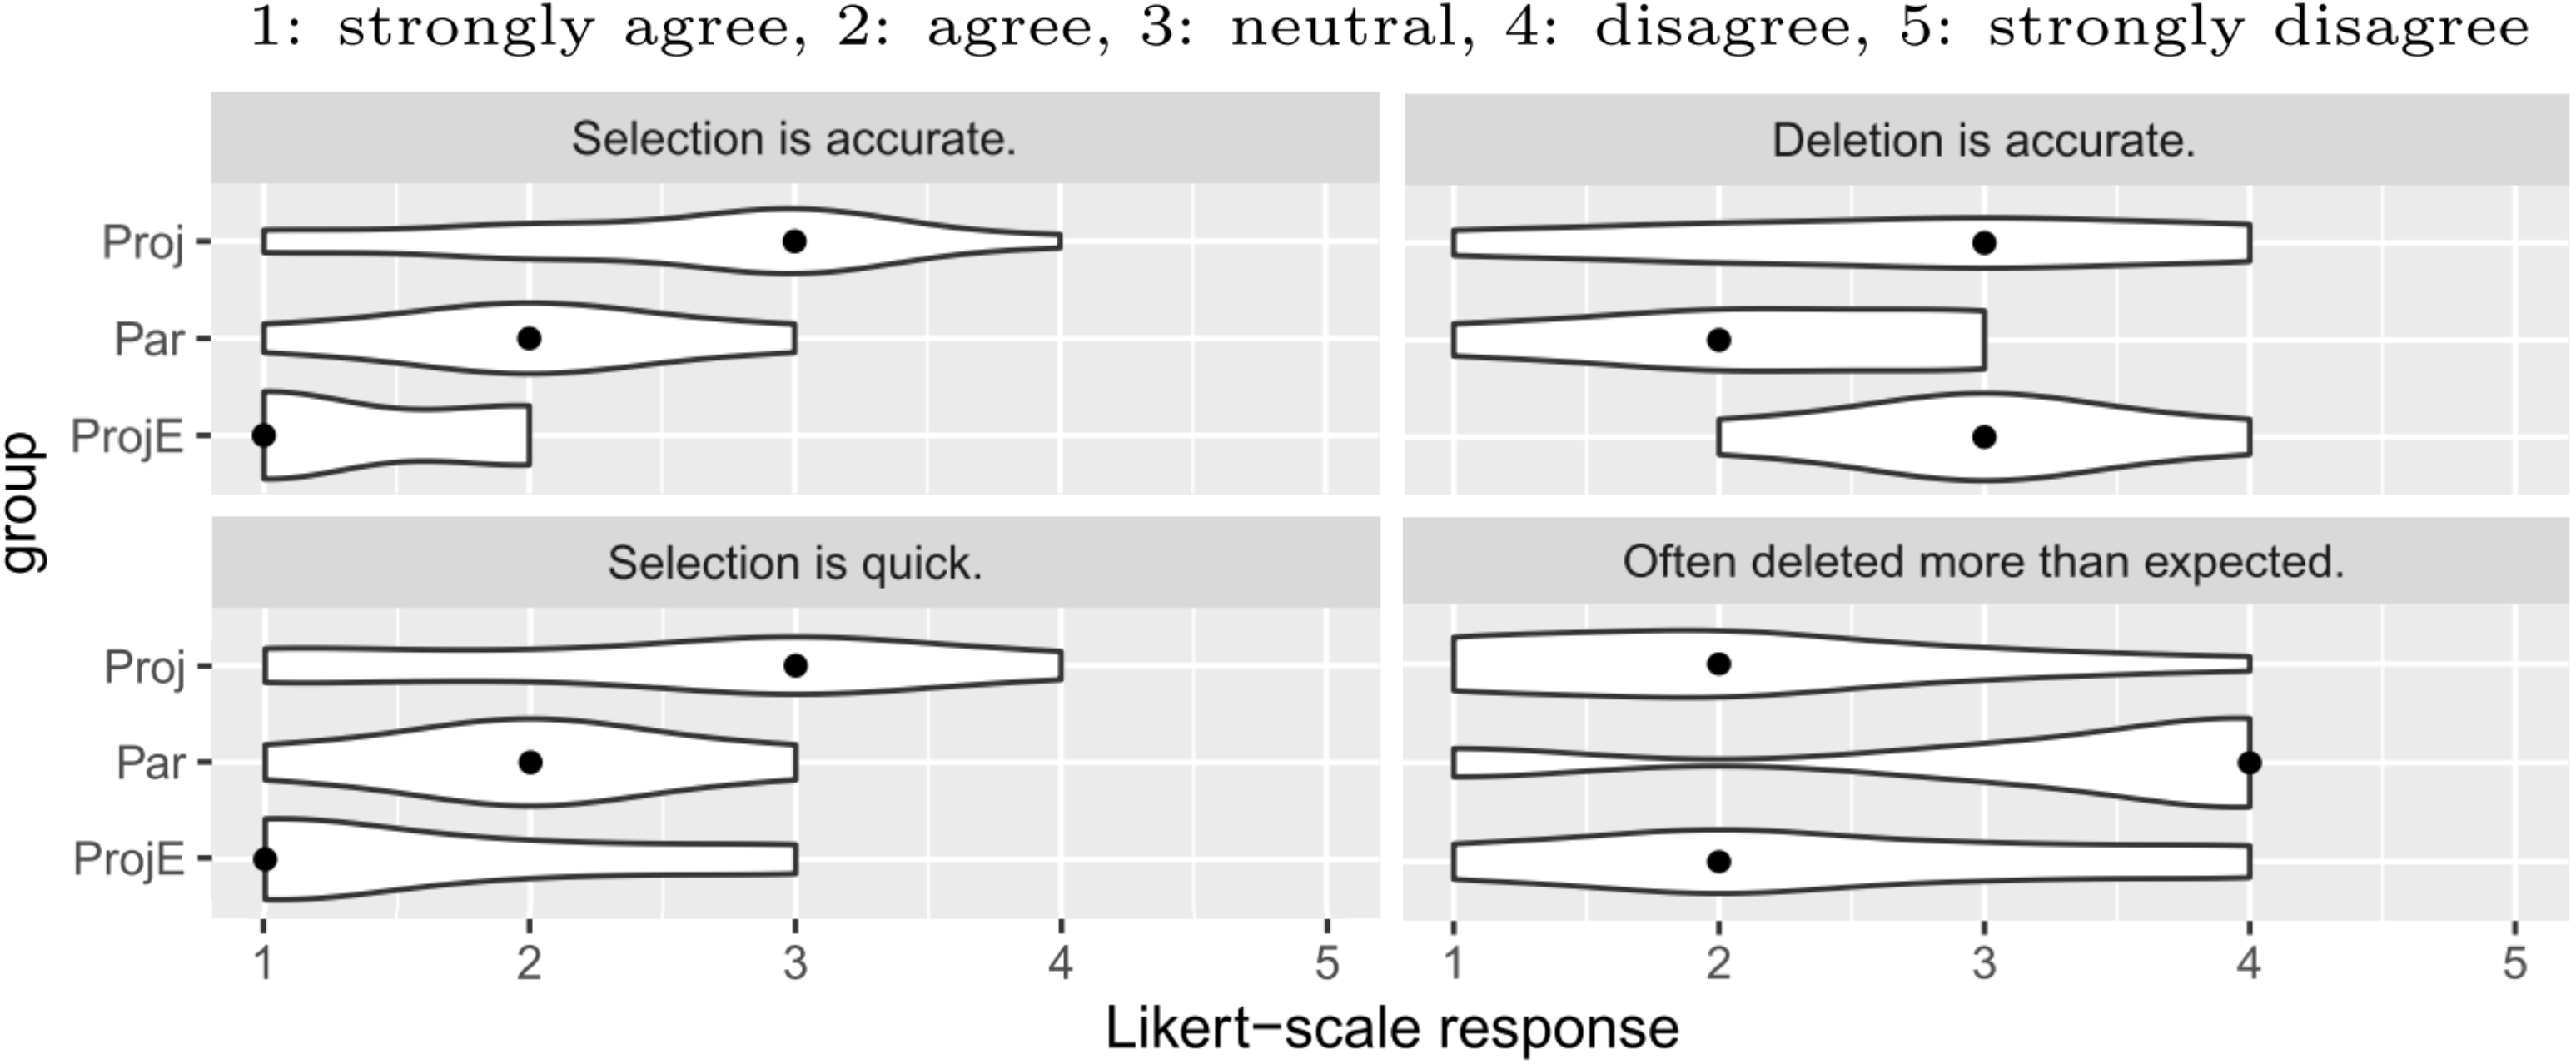
\includegraphics[width=\columnwidth]{img/mps-violin-plots.png}
  \caption{Violin plots of post-task questionnaire responses
  from a controlled user study of MPS, adapted from \cite{ProjEfficiency}.
  Each plot partitions the responses across the three study groups:
  novice MPS users (Proj), expert MPS users (ProjE),
  and text editor users (Par).
  }
  \label{fig:mps-violin-plots}
\end{figure}

Whether they are mouse-driven and block-based,
or keyboard-driven and text-like,
structure editors as a whole have suffered
from high viscosity \cite{cog-dim},
\ie, it is difficult to modify
and restructure existing code.
We believe this is a fundamental consequence
of the basic assumption that structure editors
should operate directly on the abstract syntactic structure
of a program.
% \footnote{\note{add comment here clarifying
% this is talking about pure structure editors and not
% hybrid ones and forward reference to related work}}
This assumption restricts selections to complete
program terms, a severe limitation compared to
the arbitrary range selections of text editors.
% \note{come back if there's time and talk a bit about
% Amy's thing and weave in a little more text editor vs
% structure editor dichotomy earlier}

In this paper, we describe a new approach to structure
editing, called \emph{tile-based editing}, that
recovers many of the flexible and linear editing
affordances of text editors.
The key insight is that, in order to guarantee edit state
well-formedness, it is sufficient to maintain a structure
more relaxed than the abstract syntactic structure demands,
but on which parsing is guaranteed to succeed.

Using a tile-based editor, the user manipulates
structural components called \emph{tiles} that
are shaped to fit together according to their
syntactic roles, \ala blocks in a block-based editor.
Unlike blocks, tiles directly model linear
operator sequences and facilitate left-to-right
editing using keyboard input.

Uniquely, tiles may be broken apart into
\emph{shards} as needed to specify arbitrary range
selections up to token boundaries.
Using a novel \emph{restructuring mode}, the user
may then ``cut and paste'' these selections like
in a text editor.
Unlike text-based cut-and-paste, restructuring
mode ensures you paste your selections such that
the result is a well-formed program term.

% Instead of representing the program in the language's
% abstract syntax, a tile-based editor represents it
% in a parallel tile-based syntax equipped with its own
% syntax-directed editing.

% Closely related to nested words \cite{nested-words}
% and visibly pushdown languages \cite{visibly-pushdown-langs},
% tiles encode both the linearity of sequentially
% positioned syntactic elements as well as
% their hierarchical nesting between matching sets
% of delimiters.

% \note{contributions: design and implementation of a
% minimal tile-based editor,
% formalization sketch of tile-based editing,
% discussion of how tile-based editing can be scaled up
% to more text-like interfaces like Hazel, plan to evaluate}


\section{Overview}\label{sec:overview}

% \begin{figure}
  \begin{subfigure}[c]{\columnwidth}
  \[
    \arraycolsep=3pt\begin{array}{rlrl}
        \text{pattern term} & \spat & ::= &
          \term{\ophole} ~\vert~
          \term{\svar{x}} ~\vert~
          \term{\sparen{\spat}} \\
        & & \vert &
          \term{\spat~\binhole~\spat} ~\vert~
          \term{\sprod{\spat}{\spat}} \\
        \text{expression term} & \sexp & ::= &
          \term{\ophole} ~\vert~
          \term{\snumlit{n}} ~\vert~
          \term{\svar{x}} ~\vert~
          \term{\sparen{\sexp}} \\
        & & \vert &
          % \sap{\sexp}{\sexp} ~\vert~
          \term{\sexp~\binhole~\sexp} ~\vert~
          \term{\sprod{\sexp}{\sexp}} \\
        & & \vert &
          \term{\splus{\sexp}{\sexp}} ~\vert~
          \term{\smult{\sexp}{\sexp}} ~\vert~
          \term{\sdiv{\sexp}{\sexp}} \\
        & & \vert &
          \term{\slam{\spat}{\sexp}} ~\vert~
          \term{\slet{\spat}{\sexp}{\sexp}}
    \end{array}\]
    \caption{}
    \label{fig:term-syntax}
  \end{subfigure}
  \vspace{0.4cm}

  \begin{subfigure}[c]{\columnwidth}
    \[\arraycolsep=3pt\begin{array}{rlrl}
      \text{tile sequence} & \tiles^s & ::= & \tile^s_1\dots\tile^s_n \\
      \text{pattern tile} & \tile^{\pat} & ::= &
        \tophole ~\vert~
        \soptile{\svar{x}} ~\vert~
        \soptile{\sparen{\tiles^{\pat}}} \\
      & & \vert &
        \tbinhole ~\vert~
        \sbintile{\tprod} \\
      \text{expression tile} & \tile^{\expr} & ::= &
        \tophole ~\vert~
        \soptile{\snumlit{n}} ~\vert~
        \soptile{\svar{x}} ~\vert~
        \soptile{\sparen{\tiles^{\expr}}} \\
      & & \vert &
        \tbinhole ~\vert~
        % \sap{}{} ~\vert~
        \sbintile{\tplus} ~\vert~
        \sbintile{\tmult} ~\vert~
        \sbintile{\tdiv} ~\vert~
        \sbintile{\tprod} \\
      & & \vert &
        \spretile{\tlam{\tiles^{\pat}}} ~\vert~
        \spretile{\tlet{\tiles^{\pat}}{\tiles^{\expr}}}
    \end{array}\]
    \caption{}
    \label{fig:tile-syntax}
  \end{subfigure}
  \vspace{0.4cm}
  \caption{
      Term syntax \protect\subref{fig:term-syntax} and tile syntax \protect\subref{fig:tile-syntax}
      for patterns and expressions,
      where
      $x$ ranges over variables
      % $b$ over boolean values,
      and $n$ over number literals.
  }
  \label{fig:term-tile-syntax}
\end{figure}

% \begin{figure}
  \vspace{-3px}
  \[\arraycolsep=3pt\begin{array}{rlrl}
    \text{tile sequence} & \tiles^s & ::= & \tile^s_1\dots\tile^s_n \\
    \text{pattern tile} & \tile^{\pat} & ::= &
      \ophole ~\vert~
      \svar{x} ~\vert~
      \sparen{\tiles^{\pat}} ~\vert~
      \binhole ~\vert~
      \sprod{}{} \\
    \text{expression tile} & \tile^{\expr} & ::= &
      \ophole ~\vert~
      \snumlit{n} ~\vert~
      \svar{x} ~\vert~
      \sparen{\tiles^{\expr}} \\
    & & \vert &
      \binhole ~\vert~
      % \sap{}{} ~\vert~
      \sprod{}{} ~\vert~
      \splus{}{} ~\vert~
      \smult{}{} \\
    & & \vert &
      \slam{\tiles^{\pat}}{} ~\vert~
      \slet{\tiles^{\pat}}{\tiles^{\expr}}{}
  \end{array}\]
  \caption{Tile syntax for patterns and expressions.}
  \label{fig:tile-syntax}
\end{figure}


%\note{could use Alt as toggle indicator}

We now present an example-driven overview of tile-based
editing using \tylr.

\setlength\intextsep{0pt}
\begin{wrapfigure}{r}{0.43\columnwidth}
  \centering
  \texttt{$\boldsymbol{\lambda}$ n \textbf{.} \textbf{(} n , n \textbf{)} , 1}
  \vspace{0.2cm}

  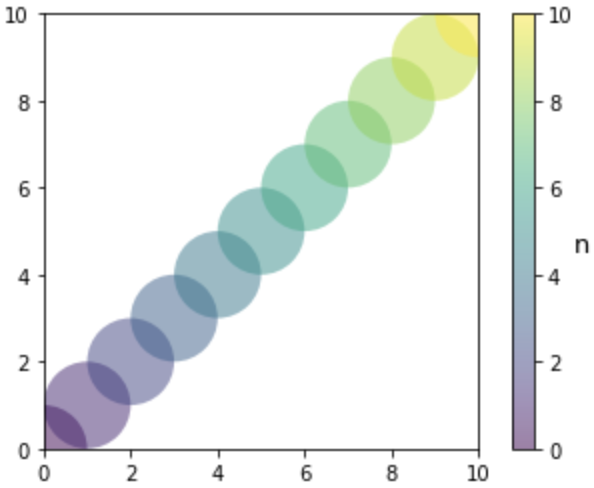
\includegraphics[width=0.43\columnwidth]{img/circles-n-n-1.png}
\end{wrapfigure}

Say we are using \tylr~ to edit a function that gets called by a
generative drawing application \cite{Processing,sns-pldi}.
The function takes an integer index and
returns a circle---represented as a pair comprising
its center point and radius---to be drawn in
the $xy$-plane for every index.
Shown above, the initial program draws unit circles
along the line $y = x$.

\subsection{Terms versus tiles}

\begin{figure}
  \centering

   \begin{subfigure}[c]{0.49\columnwidth}
      \centering
      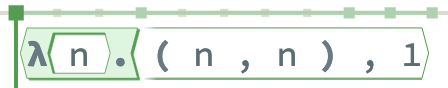
\includegraphics[width=0.9\textwidth]{img/pan-terms-0.png}
      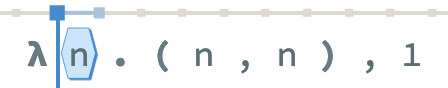
\includegraphics[width=0.9\textwidth]{img/pan-terms-1.png}
      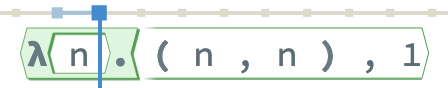
\includegraphics[width=0.9\textwidth]{img/pan-terms-2.png}
      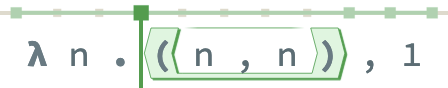
\includegraphics[width=0.9\textwidth]{img/pan-terms-3.png}
      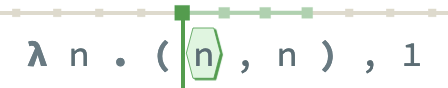
\includegraphics[width=0.9\textwidth]{img/pan-terms-4.png}
      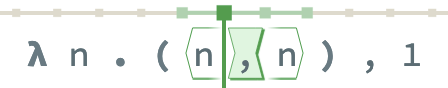
\includegraphics[width=0.9\textwidth]{img/pan-terms-5.png}
      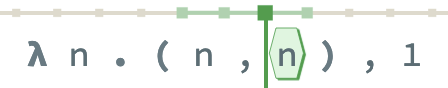
\includegraphics[width=0.9\textwidth]{img/pan-terms-6.png}
      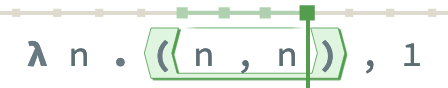
\includegraphics[width=0.9\textwidth]{img/pan-terms-7.png}
      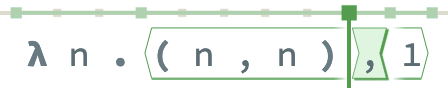
\includegraphics[width=0.9\textwidth]{img/pan-terms-8.png}
      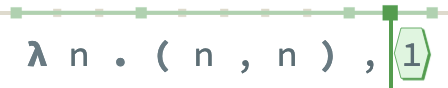
\includegraphics[width=0.9\textwidth]{img/pan-terms-9.png}
      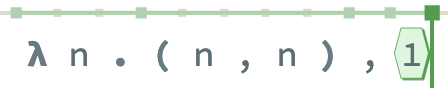
\includegraphics[width=0.9\textwidth]{img/pan-terms-10.png}
      \caption{}
      \label{fig:pan-term-view}
  \end{subfigure}
  \begin{subfigure}[c]{0.49\columnwidth}
    \centering
    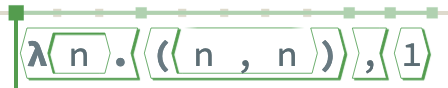
\includegraphics[width=0.9\textwidth]{img/pan-tiles-0.png}
    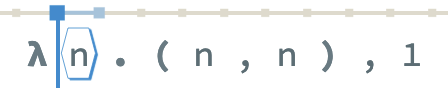
\includegraphics[width=0.9\textwidth]{img/pan-tiles-1.png}
    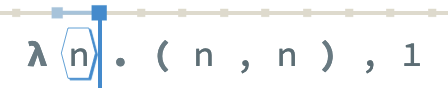
\includegraphics[width=0.9\textwidth]{img/pan-tiles-2.png}
    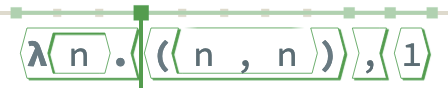
\includegraphics[width=0.9\textwidth]{img/pan-tiles-3.png}
    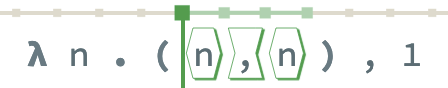
\includegraphics[width=0.9\textwidth]{img/pan-tiles-4.png}
    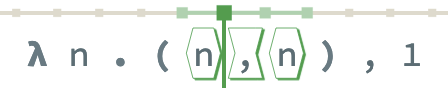
\includegraphics[width=0.9\textwidth]{img/pan-tiles-5.png}
    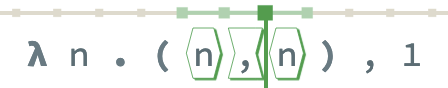
\includegraphics[width=0.9\textwidth]{img/pan-tiles-6.png}
    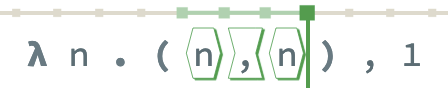
\includegraphics[width=0.9\textwidth]{img/pan-tiles-7.png}
    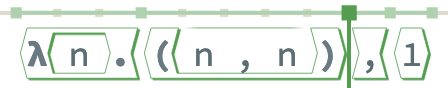
\includegraphics[width=0.9\textwidth]{img/pan-tiles-8.png}
    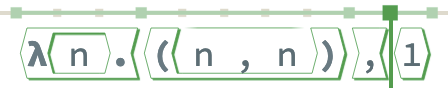
\includegraphics[width=0.9\textwidth]{img/pan-tiles-9.png}
    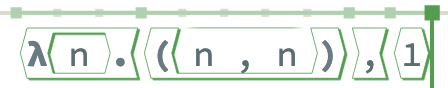
\includegraphics[width=0.9\textwidth]{img/pan-tiles-10.png}
    \caption{}
    \label{fig:pan-tile-view}
  \end{subfigure}
  \vspace{10pt}
  % \end{minipage}
  \caption{\tylr's pointing mode in \protect\subref{fig:pan-term-view} term view
  and \protect\subref{fig:pan-tile-view} tile view }
  \label{fig:pan}
\end{figure}

\begin{figure}
  \begin{subfigure}[c]{\columnwidth}
  \[
    \arraycolsep=3pt\begin{array}{rlrl}
        \text{pattern term} & \spat & ::= &
          \term{\ophole} ~\vert~
          \term{\svar{x}} ~\vert~
          \term{\sparen{\spat}} \\
        & & \vert &
          \term{\spat~\binhole~\spat} ~\vert~
          \term{\sprod{\spat}{\spat}} \\
        \text{expression term} & \sexp & ::= &
          \term{\ophole} ~\vert~
          \term{\snumlit{n}} ~\vert~
          \term{\svar{x}} ~\vert~
          \term{\sparen{\sexp}} \\
        & & \vert &
          % \sap{\sexp}{\sexp} ~\vert~
          \term{\sexp~\binhole~\sexp} ~\vert~
          \term{\sprod{\sexp}{\sexp}} \\
        & & \vert &
          \term{\splus{\sexp}{\sexp}} ~\vert~
          \term{\smult{\sexp}{\sexp}} ~\vert~
          \term{\sdiv{\sexp}{\sexp}} \\
        & & \vert &
          \term{\slam{\spat}{\sexp}} ~\vert~
          \term{\slet{\spat}{\sexp}{\sexp}}
    \end{array}\]
    \caption{}
    \label{fig:term-syntax}
  \end{subfigure}
  \vspace{0.4cm}

  \begin{subfigure}[c]{\columnwidth}
    \[\arraycolsep=3pt\begin{array}{rlrl}
      \text{tile sequence} & \tiles^s & ::= & \tile^s_1\dots\tile^s_n \\
      \text{pattern tile} & \tile^{\pat} & ::= &
        \tophole ~\vert~
        \soptile{\svar{x}} ~\vert~
        \soptile{\sparen{\tiles^{\pat}}} \\
      & & \vert &
        \tbinhole ~\vert~
        \sbintile{\tprod} \\
      \text{expression tile} & \tile^{\expr} & ::= &
        \tophole ~\vert~
        \soptile{\snumlit{n}} ~\vert~
        \soptile{\svar{x}} ~\vert~
        \soptile{\sparen{\tiles^{\expr}}} \\
      & & \vert &
        \tbinhole ~\vert~
        % \sap{}{} ~\vert~
        \sbintile{\tplus} ~\vert~
        \sbintile{\tmult} ~\vert~
        \sbintile{\tdiv} ~\vert~
        \sbintile{\tprod} \\
      & & \vert &
        \spretile{\tlam{\tiles^{\pat}}} ~\vert~
        \spretile{\tlet{\tiles^{\pat}}{\tiles^{\expr}}}
    \end{array}\]
    \caption{}
    \label{fig:tile-syntax}
  \end{subfigure}
  \vspace{0.4cm}
  \caption{
      Term syntax \protect\subref{fig:term-syntax} and tile syntax \protect\subref{fig:tile-syntax}
      for patterns and expressions,
      where
      $x$ ranges over variables
      % $b$ over boolean values,
      and $n$ over number literals.
  }
  \label{fig:term-tile-syntax}
\end{figure}

% \begin{figure}
  \vspace{-3px}
  \[\arraycolsep=3pt\begin{array}{rlrl}
    \text{tile sequence} & \tiles^s & ::= & \tile^s_1\dots\tile^s_n \\
    \text{pattern tile} & \tile^{\pat} & ::= &
      \ophole ~\vert~
      \svar{x} ~\vert~
      \sparen{\tiles^{\pat}} ~\vert~
      \binhole ~\vert~
      \sprod{}{} \\
    \text{expression tile} & \tile^{\expr} & ::= &
      \ophole ~\vert~
      \snumlit{n} ~\vert~
      \svar{x} ~\vert~
      \sparen{\tiles^{\expr}} \\
    & & \vert &
      \binhole ~\vert~
      % \sap{}{} ~\vert~
      \sprod{}{} ~\vert~
      \splus{}{} ~\vert~
      \smult{}{} \\
    & & \vert &
      \slam{\tiles^{\pat}}{} ~\vert~
      \slet{\tiles^{\pat}}{\tiles^{\expr}}{}
  \end{array}\]
  \caption{Tile syntax for patterns and expressions.}
  \label{fig:tile-syntax}
\end{figure}


% \note{maybe forward reference alternative choices not skipping tokens}
Panning the cursor over the program in \tylr,
as shown in Figure \ref{fig:pan-term-view},
reveals the program structure as
governed by \tylr's \emph{term syntax},
the relevant subset of which is shown in
Figure \ref{fig:term-syntax}.
For example, the first edit state in Figure \ref{fig:pan-term-view}
shows the top-level function---an expression term as
indicated by the green coloring---binding
the pattern variable \code{n} and returning an indexed circle.
Notice how every term has a convex hexagonal shape.

Highlighted within each term is a substructure called a \emph{tile};
with respect to the containing term, we say it is the term's \emph{root tile}.
Each term's root tile encompasses all root-level tokens used to
represent the term, along with children of the term that the tokens
delimit on both sides---such children we call \emph{bidelimited}.
For example, in the first edit state of
Figure \ref{fig:pan-term-view}, observe how the function's highlighted
tile spans the function's tokens \code{$\boldsymbol{\lambda}$}
and \code{\textbf{.}\vphantom{$\boldsymbol{\lambda}$}}
as well as the bidelimited pattern child; however, it does not
extend to the \emph{unidelimited} body child.

Holding Alt/Option while panning the cursor, this time in
Figure \ref{fig:pan-tile-view}, reveals the program structure
as governed by \tylr's \emph{tile syntax},
shown in Figure \ref{fig:tile-syntax}.
Tiles enjoy a flatter structure compared to the
strictly hierarchical terms.
Notice in the first edit state of Figure \ref{fig:pan-tile-view},
for example, how the tiles comprising the function body
are siblings with the function term's root tile.
The \emph{tips} of a tile indicate its syntactic
role in the tile sequence as a(n):
\toptile{operand}, \tpretile{prefix operator},
\tposttile{postfix operator}, or \tbintile{infix operator}.

Where traditional structure editors model their edit states
using the strictly hierarchical term syntax,
% \footnote{
%   Technically, most other structure editors model their edit states
%   in terms of the language's abstract syntax, whereas the
%   term syntax used here is more akin to the concrete syntax,
%   but the important point is that they are both strictly hierarchical.
% }
\tylr~ instead models its edit state using the flatter
tile syntax, precedence-parsing the tile structure
as needed to produce the term structure.
Indeed, the term structure shown in Figure \ref{fig:pan-term-view}
is simply a decoration overlaid atop the actual tile
structure shown in Figure \ref{fig:pan-tile-view}.
Moving forward, we will refer to structure editors
with term-structured edit states as \emph{term-based editors}.

\subsection{Opseqs \& holes}

The edit states shown in Figure \ref{fig:pan} are in
\emph{pointing mode}, \tylr's default editing mode.
Much like how a text editor's cursor points at positions
between characters in its default mode, \tylr's default
cursor points at positions between tiles.
% \note{note how they are explicitly indicated in above
% the terms/tiles, the local cursor positions for the current tile
% sequence are shown, that we can speak meaningfully of the
% sort of a cursor position, maybe forward reference that
% this will be useful for explaining how selecting works}
\tylr's central guarantee is: if you are in pointing mode,
then you have a well-formed program term.

Simply maintaining a well-formed tile structure
according to the tile syntax alone, however, is
not sufficient to uphold this guarantee.
The generic sequential structure of tile sequences
simplifies how we define edit operations, but
does not guarantee that the tiles represent a well-formed
\emph{operator sequence}, or \emph{opseq} for short.
The qualifications for a tile sequence to an opseq
enjoy a simple physical metaphor:
\begin{enumerate}
\item[(1)] every tile \emph{fits} its neighbors:
  if a pair of tips meet, they look like $\ltiletip\ltiletip$
  or $\rtiletip\rtiletip$; and
\item[(2)] every tile sequence is \emph{convex}:
  it is nonempty, the first tile's left tip $\ltiletip$
  points left, and the last tile's right tip $\rtiletip$
  points right.
\end{enumerate}
If \tylr~ maintains well-formed opseqs in pointing mode, then we have
our guarantee, since precedence-parsing is total on opseqs.

For this reason, \tylr~ automatically inserts
and removes placeholder tiles called \emph{holes}
as we edit to maintain opseq structure.
There are two kinds of holes:
\emph{operand holes} \optile{\ophole}
and \emph{operator holes} \bintile{\binhole}.
We will soon see a number of examples of
automatic hole fixing as we turn our attention
to editing.

% \note{also mention right bias of term view (for simplicity)}

% \note{following sentence too vague, couch in concrete example,
% be more clear about highlighting the root vs the whole tile,
% probably refer explicitly to tile syntax earlier to make it
% more precise}
% Highlighted at the root of every term is a structure called
% a \emph{tile}.
% The tile encompasses all tokens used to represent
% the root form of the term (e.g., \texttt{1} for a number literal,
% $\lambda$ and \texttt{.} for lambda terms,
% \texttt{(} and \texttt{)} for parenthesized terms) along with
% all children terms delimited on both sides (\eg,
% the bidelimited pattern child \texttt{n} of the lambda term,
% the bidelimited expression child \texttt{n , n} of
% the parenthesized term).

% Tiles are closely related to nested words \note{cite} and
% visibly pushdown languages \note{cite}, which we discuss
% further in Section \ref{sec:related-work}.

\subsection{Inserting and removing tiles} \label{sec:inserting-removing}
By having us edit the tile structure, and only
indirectly propagate those edits to the term structure,
\tylr~ recovers many of the flexible editing affordances to
which we are accustomed in text editors.

\setlength\intextsep{0pt}
\begin{wrapfigure}{r}{0.08\columnwidth}
  \centering
  \hspace*{-0.07\columnwidth}
  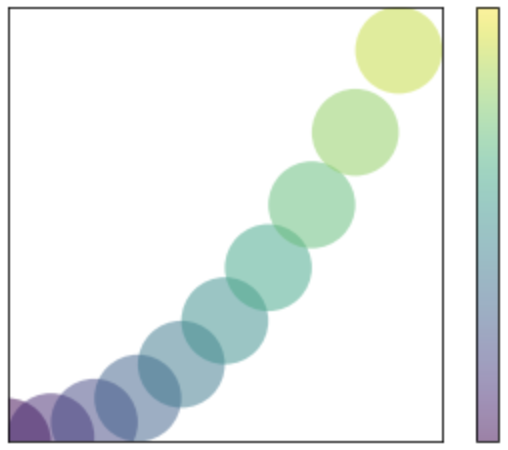
\includegraphics[width=0.15\columnwidth]{img/circles-parabola.png}
\end{wrapfigure}

\paragraph{Leaf tiles}
We update the function to
draw circles along the parabola $y = x^2/9$,
as depicted on the right,
using the edit sequence below.

\begin{figure}[h]
  \centering
% \begin{minipage}[t]{0.2\columnwidth}
%   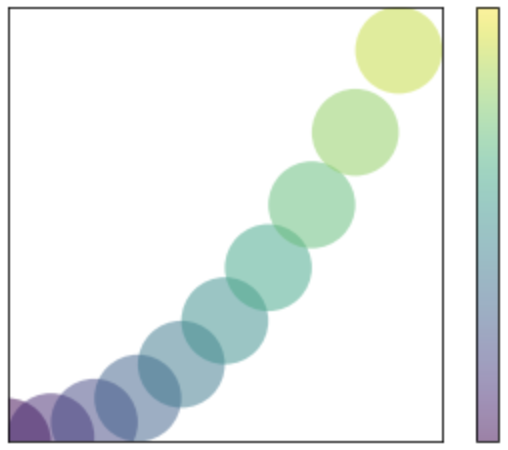
\includegraphics[width=\textwidth]{img/circles-parabola.png}
% \end{minipage}
% \hfill
% \begin{minipage}{0.65\columnwidth}
  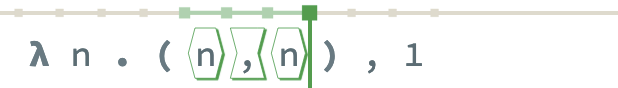
\includegraphics[width=0.7\columnwidth]{img/linear-insertion-0.png}
  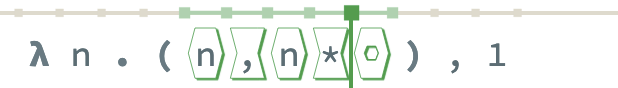
\includegraphics[width=0.7\columnwidth]{img/linear-insertion-1.png}
  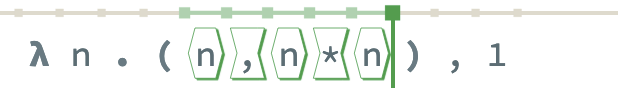
\includegraphics[width=0.7\columnwidth]{img/linear-insertion-2.png}
  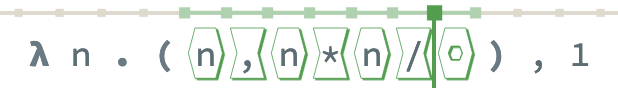
\includegraphics[width=0.7\columnwidth]{img/linear-insertion-3.png}
  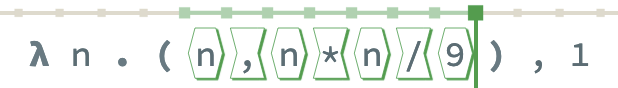
\includegraphics[width=0.7\columnwidth]{img/linear-insertion-4.png}
  % \caption{Inserting}
% \end{minipage}
\end{figure}

\setlength\intextsep{0pt}
\begin{wrapfigure}{r}{0.08\columnwidth}
  \centering
  \hspace*{-0.07\columnwidth}
  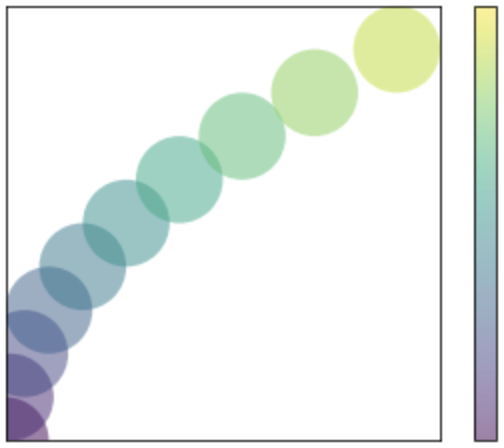
\includegraphics[width=0.15\columnwidth]{img/circles-parabola-transpose.png}
\end{wrapfigure}

If we decided now to draw circles along the reflected
parabola $x = y^2/9$, we could similarly remove the inserted
tiles right-to-left from the $y$-coordinate and re-insert
them in the $x$-coordinate.

\note{figure of linear removal}

These simple editing workflows are not trivial
in traditional term-based editors because,
from the perspective of the AST, linear construction of
operator sequences is a complex, context-sensitive operation.
Existing structure editors either embrace strictly tree-based
construction of operator sequences \cite{scratch};
defer to text at the expression level \cite{Cornell,greenfoot},
recovering linearity at the cost of structure;
or solve the problem at the cost of complexity
\cite{GrammarCells}.
In contrast, tiles combined with automatic hole fixing
make it easy to define linear editing operations
without compromising structure.

% \note{add one more final snapshot in term view, showing
% how tylr parses precedence/associativity}

% \note{pause after constructing the times and note how
% precedence is re-parsed}

% \note{note that this is insertion, not ``hole filling'' as
% it is traditionally conceived in structure editors}

% \note{insert a comment somewhere about no performance claims}

% \note{review side transforms and make sure I'm not BSing}

% \note{figure out where to talk about hole insertion based on tips
% somewhere here}

% \tylr~ takes a different approach to this problem.
% Where traditional structure editors simply expose editing
% operations acting directly on the abstract syntactic struture
% of a program, \tylr~ presents the program in a separate
% concrete syntax with its own syntax-directed editing operations.
% \note{
%   talk about tile syntax show in Figure \ref{fig:tile-syntax},
%   note linearity
% }
% Like text, \tylr's concrete syntax gives you ``flattened''
% representation of your program that can be edited in a linear fashion.
% Unlike text, the concrete syntax maintains hierarchies of
% bidelimited children and can always be parsed into
% the abstract syntax, provided that the structure first undergoes
% a hole fixing pass in which holes are inserted and removed
% as needed. \note{need more context about tiles + bidelimited, bring
% back some old words about abstract syntactic structural units
% as opposed to concrete syntactic structural units}

% \note{perhaps go back to editor syntax terminology}

\begin{figure*}
  \begin{tabular}{cp{0.7\textwidth}}
  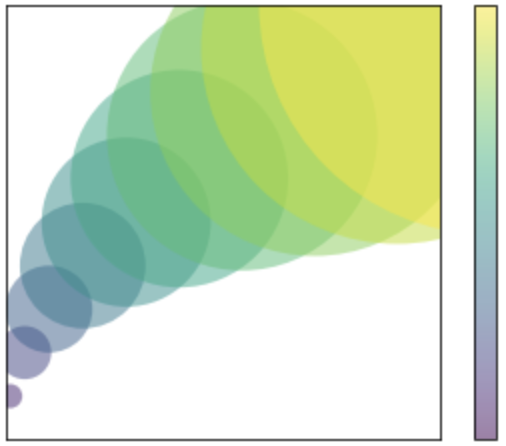
\includegraphics[width=0.1\textwidth]{img/circles-parabola-grow-1.png}
  &
  {
    \begin{align*}
      & \texttt{$\lambda$ n . let x , y = \_|in ( n * n / 9 , n ) , 1} \\
      & \texttt{$\lambda$ n . let x , y = \_|in|( n * n / 9 , n ) , 1} \\
      & \texttt{$\lambda$ n . let x , y = [in]( n * n / 9 , n ) , 1} \\
      & \texttt{$\lambda$ n . let x , y = ( n * n / 9 , n )[in], 1} \\
      & \texttt{$\lambda$ n . let x , y = ( n * n / 9 , n )|in \_ , 1} \\\\
      & \texttt{$\lambda$ n . let x , y = ( n * n / 9 , n|) in x , y , 1 } \\
      & \texttt{$\lambda$ n . let x , y = ( n * n / 9 , n|)|in x , y , 1 } \\
      & \texttt{$\lambda$ n . let x , y = |(|n * n / 9 , n[)]in x , y , 1 } \\
      & \texttt{$\lambda$ n . let x , y = |(|[)]n * n / 9 , n in x , y , 1 } \\
      & \texttt{$\lambda$ n . let x , y = [(][)]n * n / 9 , n in x , y , 1 } \\
      & \texttt{$\lambda$ n . let x , y = n * n / 9 , n in [(][)]x , y , 1 } \\
      & \texttt{$\lambda$ n . let x , y = n * n / 9 , n in ( x , y[)], 1 } \\
      & \texttt{$\lambda$ n . let x , y = n * n / 9 , n in ( x , y|) , 1 } \\\\
      & \texttt{$\lambda$ n . let x , y = n * n / 9 , n in ( x , y ) ,|x + y } \\
      & \texttt{$\lambda$ n . let x , y = n * n / 9 , n in ( x , y ) ,|(|[)]x + y } \\
      & \texttt{$\lambda$ n . let x , y = n * n / 9 , n in ( x , y ) ,|(|x + y[)]} \\
      & \texttt{$\lambda$ n . let x , y = n * n / 9 , n in ( x , y ) , ( x + y|)} \\
      & \texttt{$\lambda$ n . let x , y = n * n / 9 , n in ( x , y ) , ( x + y )|} \\
      & \texttt{$\lambda$ n . let x , y = n * n / 9 , n in ( x , y ) , ( x + y ) /|\_} \\
      & \texttt{$\lambda$ n . let x , y = n * n / 9 , n in ( x , y ) , ( x + y ) / 4|}
    \end{align*}
  }
  \end{tabular}
\end{figure*}

\begin{figure*}
  \begin{tabular}{cp{0.7\textwidth}}
  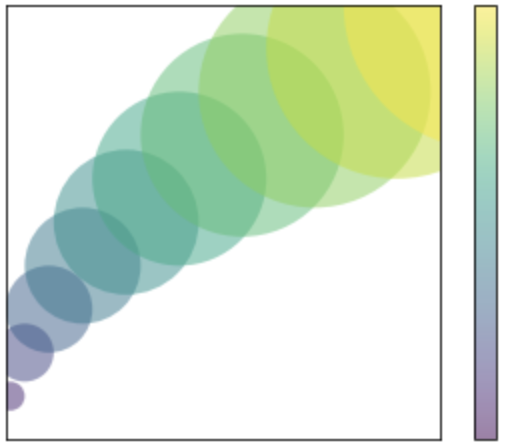
\includegraphics[width=0.1\textwidth]{img/circles-parabola-grow-2.png}
  &
  {
    \begin{align*}
      & \texttt{$\lambda$ n . let x , y = n * n / 9 , n|in ( x , y ) , n / 3} \\
      & \texttt{$\lambda$ n .|let x , y =|n * n / 9 , n[in] ( x , y ) , n / 3} \\
      & \texttt{$\lambda$ n . n * n / 9 , n|\_ ( x , y ) , n / 3} \\
      & \texttt{$\lambda$ n . n * n / 9 , n \_ (|x , y ) , n / 3} \\
      & \texttt{$\lambda$ n . n * n / 9 , n \_ (|x , y|) , n / 3} \\
      & \texttt{$\lambda$ n . n * n / 9 , n \_ (|\_ ) , n / 3} \\
      & \texttt{$\lambda$ n . n * n / 9 , n [(]|)|, n / 3} \\
      & \texttt{$\lambda$ n .[(]n * n / 9 , n|)|, n / 3} \\
      & \texttt{$\lambda$ n .|( n * n / 9 , n ), n / 3}
    \end{align*}
  }
  \end{tabular}
\end{figure*}

\paragraph{Non-leaf tiles}
While insertion and removal of leaf tiles closely mimics the
text editing experience, this begins to change as we turn our
attention to non-leaf tiles.
For example, consider below how we would remove the parentheses
wrapping the origin coordinates in \tylr.

\note{figure}

Where a text editor would simply remove the closing parenthesis
on the first Backspace, leaving us with a syntax error,
\tylr~ first enters an intermediate state in which it has
"picked up" the closing parenthesis and highlighted the
matching opening parenthesis.
Pressing Backspace again then removes both parentheses.

This intermediate state is called \emph{restructuring mode},
and we picked up the closing parenthesis into the \emph{backpack};
we will soon discuss these at greater length.
For now, notice how restructuring mode served as a
sort of confirmation dialog, showing us that removing
the token on which we hit Backspace would require
deleting other tokens.
We believe such explicit confirmation is important to
prevent ``spooky action at a distance'', especially
in light of the MPS user data discussed in Section \ref{sec:intro}.

Now consider how we might re-insert the parentheses
around the origin coordinates.

\note{figure}

\noindent
In a dual fashion to removal, inserting
an opening parenthesis enters restructuring mode with its
matching closing parenthesis in the backpack.
Restructuring mode then allows us to move the parenthesis
to the right and put it down.
Notice the similarity to the text editing experience,
which has an invoke-then-configure flow, whereas a typical
structure editor would require you to select the body before
parenthesizing, forcing preemptive configuration before
invocation.

MPS supports a similar editing flow for parentheses in particular,
but not any other syntactic forms also with matching delimiters.
In contrast, as we will see next, \tylr~ has well-defined
restructuring behavior for arbitrary range selections.

\subsection{Selecting and restructuring} \label{sec:selecting-restructuring}

Using the arrow keys while holding
Shift enters \tylr's \emph{selecting mode}.

\note{figure}

Selecting mode lets us specify arbitrary range selections up
to token boundaries.
Notice how, when a tile is divided by a selection boundary,
it is disassembled into individual \emph{shards}.
Then, once they are all within or without the selection,
the shards are reassembled into the original tile.

Collectively we call tiles and shards \emph{pieces},
a sequence of pieces a \emph{segment}.
A segment containing only tiles is called \emph{intact},
otherwise \emph{cracked}.
We may understand restructuring mode, not simply as a tile insertion
and removal aid, but more generally as a structured variant of
cut-and-paste of selected segments, regulated by their intact versus
cracked structure.

% Tiles not only simplify linear \emph{insertion} in a structured
% context but also enable text-like \emph{selecting}
% and \emph{restructuring} (e.g. cut and paste) of existing code.
% While the former problem is relatively well-studied
% \note{cite MPS, modeless structure editing},
% almost no attention has been paid to the latter.
% In particular, all prior structure editors restrict
% structured selections to complete concrete syntactic terms,
% a severe limitation compared to the arbitrary range
% selections of text editors.

% \tylr~ recovers much of this lost flexibility.
% Using \tylr's \emph{selecting mode}, you can
% make arbitrary range selections up to token boundaries,
% disassembling tiles into \emph{shards} as needed.
% Using \tylr's \emph{restructuring mode},
% you can pick up your selections into your
% \emph{backpack} and put them down elsewhere,
% à la cut-and-paste using the clipboard.
% Unlike the usual clipboard, however,
% your backpack is structure-aware and guides your
% movement toward valid paste targets, \ie,
% you can only put down your backpack's contents
% where the result can be reassembled into well-formed tiles.

% \note{add another paragraph header focused on selecting}

% \note{see if I can talk about intact vs cracked selections here,
% perhaps by changing the direction of the first selection and
% introducing shards when right parens get selected}

% \note{so far we have been in pointing mode...}

% \setlength\intextsep{0pt}
% \begin{wrapfigure}{r}{0.08\columnwidth}
%   \centering
%   \hspace*{-0.07\columnwidth}
%   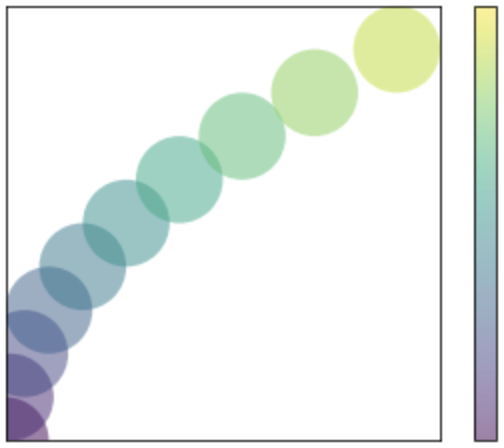
\includegraphics[width=0.15\columnwidth]{img/circles-parabola-transpose.png}
% \end{wrapfigure}

\paragraph{Restructuring with a full backpack}
In Section \ref{sec:inserting-removing}, we updated the circle drawing tracing the
parabola $y = x^2/9$ to its reflection $x = y^2/9$ by deleting
and re-inserting tiles.
Alternatively, we could have selected the inserted tiles---an impossible
selection in a term-based editor---and used
restructuring mode to move them. \note{need to add more steps below}
% Say you update your circle drawing
% to its transposition, i.e., draw the circles along
% the parabola $x = y^2/9$.
% Entering selecting mode, you anchor the selection's right
% end and move left to select the tiles you just
% inserted in the $y$-coordinate---an impossible
% selection in prior structure editors.

\begin{figure}[h]
  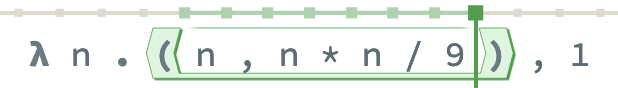
\includegraphics[width=0.65\columnwidth]{img/selection-whole-0.png}
  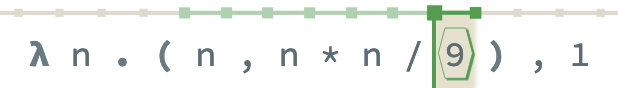
\includegraphics[width=0.65\columnwidth]{img/selection-whole-1.png}
  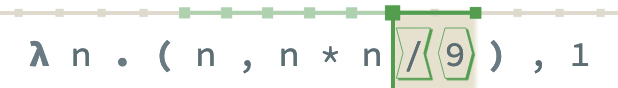
\includegraphics[width=0.65\columnwidth]{img/selection-whole-2.png}
  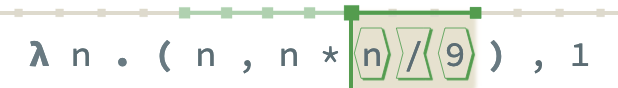
\includegraphics[width=0.65\columnwidth]{img/selection-whole-3.png}
  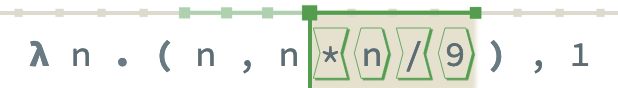
\includegraphics[width=0.65\columnwidth]{img/selection-whole-4.png}
\end{figure}
% You then pick it up into your backpack to enter
% restructuring mode.
% Moving left to the $x$-coordinate and putting down
% the selection completes the desired transformation.

% \noindent
% \begin{tabular}{cp{7cm}}
% 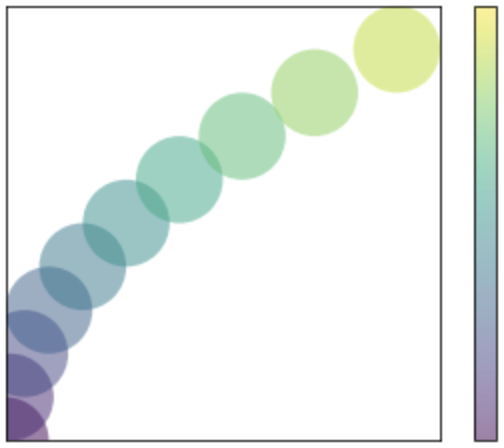
\includegraphics[width=2cm]{img/circles-parabola-transpose.png}
% &
% {
% \begin{align*}
%   & \texttt{$\lambda$ n . ( n , n[* n / 9]) , 1} \\
%   & \texttt{$\lambda$ n . ( n ,[* n / 9]n ) , 1} \\
%   & \texttt{$\lambda$ n . ( n[* n / 9], n ) , 1} \\
%   & \texttt{$\lambda$ n . ( n|* n / 9 , n ) , 1}
% \end{align*}
% }
% \end{tabular}

% \note{define intact selections}

We say that the backpack is \emph{full} whenever
its contents are, or could be assembled into, an intact selection.
If the backpack is full, then we may move freely,
since we may insert a selection of whole tiles anywhere
without compromising the existing shard-balanced structure.

% \note{define cracked selections}

Often, however, the backpack's contents are not an intact
selection, nor can they be assembled into one, as we observed
in the parentheses insertion and removal examples in Section \ref{sec:inserting-removing}.
In that case, we say that the backpack is \emph{hungry}...

\paragraph{Restructuring with a hungry backpack}

Now we would like the circles' radii to grow
with their origin coordinates; accordingly,
as shown at the top of Figure ??,
we have inserted
a let tile introducing variables \code{x} and \code{y}
in the function body.
Our next task is to restructure our code so that \code{x}
and \code{y} are bound to the origin coordinates
\code{( n * n / 9 , n )} currently in the body of the let term.
We select the \code{in} delimiter,
disassembling the \code{let}-tile in the process;
move right once; and put it down,
upon which \tylr~ reassembles the \code{let}-tile
and returns us to pointing mode.

\begin{figure}[h]
  \centering
  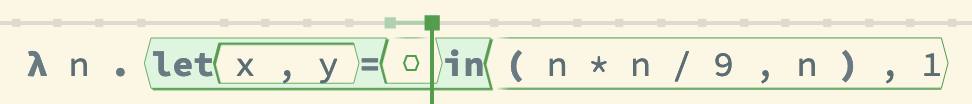
\includegraphics[width=0.9\columnwidth]{img/placeholder-restructuring-hungry.png}
\end{figure}

% \note{figure out a way to introduce hole fixing, why operand hole
% disappears rather than operator hole being introduced, might be
% here or worked in before}

% \note{when discussing hole minimality, distinguish from other
% interfaces where you insert holes manually, so you shouldn't
% remove automatically}

% Your editing workflow was similar to what you might
% have done in a text editor---delete the \texttt{in}
% delimiter, move right, re-type---except that \tylr~
% skipped all cursor positions within the parentheses tile
% when you moved right.
Notice that we skipped all cursor positions within
the parentheses tile when we moved right.
The \code{in}-shard in our backpack could not be assembled into
a whole tile on its own, meaning at least one matching shard---in
this case, \code{let x , y =}---was
anchored within the current tile sequence.
This restricted our movement of the \texttt{in}-shard
to cursor positions of the same sequence,
as placing it in any other position would
violate proper nesting of matching shards.

% \note{add back some discussion comparing to text editing
% and other structure editors;
% similarity with text workflow,
% while making it more efficient + less cognitive load;
% other structure editors would force you to translate
% edits into term-based selections, can be awkward or
% not the most efficient in terms of selection size}

We call the backpack full or hungry as a way
to narrativize its control of our movement.
When the backpack is full, it is satisfied
and lets us move freely and leisurely through
our code.
When the backpack is hungry, it accelerates our
movement through the current tile sequence
in its impatience to end its hunger, which can happen in one of two ways.
Either, like in the last example, we can empty the backpack,
freeing it of all earthly possessions and desires;
or we may feed it.

% \note{add forward reference to discussing alternatives, eg,
% not skipping cursor positions}

% We hypothesize that such a restriction would lead to both greater
% editing efficiency and reduced cognitive load compared to
% text editing on similar tasks.

% We hypothesize that such a restriction would easy to learn
% given
% \begin{itemize}
% \item be easy to learn, given the workflow similarity to text editing;
% \item lead to greater editing efficiency than text editing due to
%     the fewer keypresses needed to reach valid paste/restructure targets; and
% \item reduce cognitive load compared to text editing because you
%     no longer need to count delimiters to ensure you have reached
%     a valid paste/restructure target.
% \end{itemize}

\paragraph{Feeding a hungry backpack}
Now we rewrite the radius in terms of the variables
\code{x} and \code{y}, as shown at the top of
Figure ??.
Along the way, however, we forget to parenthesize
the origin coordinates.
We also notice that the parentheses in the definition
of the \code{let}-tile are now redundant and decide
to recycle them.
At this point the backpack is hungry and restricts
our movement to the tile sequence within the
let definition.
Instead of emptying our backpack like in the
last example, this time we move over to the
left parenthesis and pick it up as well.
Now our backpack is full, as it carries both shards
needed to assemble a parentheses tile, and we may
now move freely out of the let definition
to put down the parentheses around the origin coordinates.
% \note{add labels to edit states,
% label sentences here}

% Say you have filled the hole in Figure ?? with
% the variables \texttt{x} and \texttt{y} you defined
% in the previous example, as shown in Figure ??.
% Upon reviewing the term structure, however, you
% discover that pairs are right-associative in \tylr,
% so you need to wrap \texttt{x , y} in parentheses
% in order to satisfy the expected return type.
% \note{maybe just say we've created a triple but we
% really want a pair of a pair on left}
% You also notice that the parentheses in the definition
% of the \texttt{let} tile are now redundant
% and decide to recycle them.
% You move your cursor to the right parenthesis,
% select it, and pick it up into your backpack.
% At this point your backpack is hungry and restricts
% your movement to the tile sequence within the
% let definition.
% Instead of emptying your backpack like in the
% last example, this time you move over to the
% left parenthesis and pick it up as well (Figure ??).

% \note{make note of pattern not having parentheses}

% When your backpack carries multiple selections,
% it dictates the order in which you can put them down.
% Most of the time it behaves like a stack, putting
% down first the last picked up selection; we discuss
% deviations

Now your backpack is full, as it carries both shards
needed to assemble a whole parentheses tile,
and you may move freely again.
You carry the parentheses over to the body of the
let term and wrap \texttt{x , y} to complete your
restructuring.

The last example showed how \tylr~ lets you carry \emph{multiple}
related range selections in your backpack.
This ability vastly improves your selecting precision
compared to prior designs.
From the perspective of the term syntax,
where other structure editors force you to select
complete subtrees, \tylr~ lets you cut out individual
\emph{nodes} of the tree and splice them back in
elsewhere.
% \note{either remove this or rewrite when it's more as
% an emergent phenomenon}

% \paragraph{Staging tile insertion}
% \note{maybe just call restructuring on insertion}

% \note{add connecting intro connecting to node-centric perspective}
% Say you have completed an initial draft of your goal program,
% where each circle's radius is the sum of its origin
% coordinates, as shown in Figure ??.
% You discover, however, that the circles are so large that
% they fill your viewport, so you would like to make them smaller.
% You begin by inserting a left parenthesis
% before \texttt{x + y}, your intention being to wrap
% the sum and divide it by a constant factor.
% Upon this insertion, \tylr~ automatically enters
% restructuring mode with the matching right parenthesis
% in your backpack.
% You move right, put down the right parenthesis,
% and complete your desired transformation.

% \note{add discussion}

% \note{note how other structure editors force you to select
% child first before constructing}

\paragraph{Picky eating}
Not all selections can be picked up.
We call the cursor positions marking the ends of a selection
the selection's \emph{caps}.
So far we have only encountered selections with caps
of the same sort.
Your backpack is a picky eater in that
it will refuse to carry any selections with caps of
different sort.

Consider, for example, the following selection:

\note{example fig}

\noindent
The left cap is pattern-sorted while the right cap
is expression-sorted, as indicated by the two-toned
broken overline.
Picking up this selection would bring together
tiles of different sort, violating \tylr's edit
state well-formedness, so you are prevented from doing so.

% \note{show small inline example of selecting
% selection with caps of different sort}

% \note{show small inline example of selection
% with pattern caps cutting across expressions}

\subsection{Removing selections}

Lastly, we turn our attention to selection removal,
generalizing our understanding of tile removal
in pointing mode as discussed in
Section \ref{sec:inserting-removing}.
% Pressing Backspace on a selection
% has one of two effects:
% (1) if it is intact, remove the selection
%     and return to pointing mode;
% (2) otherwise, enter restructuring mode with
%     the smallest containing same-sort-capped selection
%     in your backpack.
% Pressing Backspace again in restructuring mode
% removes all highlighted tiles and selections.
Removing a selection works in one of two ways,
depending on whether the selection is intact or cracked.

\begin{figure}[h]
  \centering
  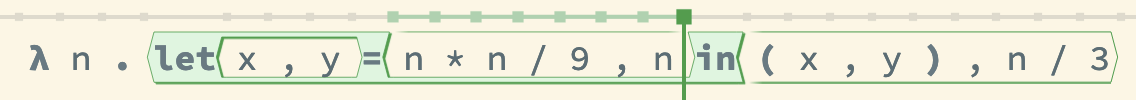
\includegraphics[width=\columnwidth]{img/test-wide.png}
\end{figure}

\paragraph{Removing intact selections}
Say we fiddled some more with our last circle drawing
and discovered a similar drawing we like a bit better,
shown in Figure ??.
Upon reviewing our code, we realize we no longer
need to define variables \code{x} and \code{y},
since they are each used only once, and can inline
their definition.
We begin by removing the uses of \code{x} and \code{y},
selecting \code{x , y} in the body of the \code{let}
term and hitting Backspace.
In this case, because our selection is intact, \tylr~
immediately removes our selection, as we might
expect from our experience with text editors.

\paragraph{Removing cracked selections}
Now we would like to remove the \code{let}-tile,
but we want to preserve its definition so we
can inline it.
We select the \code{in}-shard and hit Backspace.
Because our selection is cracked, removing
our selection would require also removing the
matching \code{let}-shard that we have not
explicitly selected ourselves.

\tylr~ does not remove both shards immediately but
instead enters restructuring mode, giving us the option
to move the \code{in}-shard like in Section \ref{sec:selecting-restructuring},
or to proceed with removal of the highlighted pieces
like in Section \ref{sec:inserting-removing}.
We confirm the total removal by hitting Backspace again,
leaving behind the let definition and body
separated by an operator hole.

% In general, pressing Backspace on a selection
% has one of two effects:
% \begin{enumerate}
%   \item[(1)] remove the selection if it is intact
%     and return to pointing mode;
%   \item[(2)] otherwise entering restructuring mode with
%     the smallest containing selection with same-sort caps
%     in your backpack.
% \end{enumerate}
% Pressing Backspace again in restructuring mode
% removes all highlighted tiles and selections.
% In sum: if your selection is intact then you can
% remove it with a single tap of Backspace; otherwise
% you need to double tap.

% If your selection is fragmentary, then removing
% your selection would require also removing matching shards
% that you have not explicitly selected yourself.
% \tylr~ does not remove the implicit selections immediately
% but instead enters restructuring mode as a staging
% ground in which you may confirm the total removal
% by hitting Backspace again (or otherwise proceed
% with restructuring).
% \note{draw parallel with staged insertion}
% In sum: if your selection is intact then you can
% remove it with a single tap of Backspace; otherwise
% you need to double tap.


\paragraph{Removing in pointing mode}
Finally, it remains to restructure the parentheses
so that they wrap the origin coordinates.
This time, instead of first explicitly specifying a selection,
you position your cursor after the left parenthesis
and hit Backspace within pointing mode.
\tylr~ treats this input simply as a shortcut for selecting the
token immediately to your left and then hitting Backspace.
In this case, the token to your left is a parenthesis
shard that forms a fragmentary selection, so you
enter restructuring mode with the parenthesis in tow.
You move left to the other side of the origin coordinates,
then put down the parenthesis to complete the transformation.

% \note{more words here to wrap up}


%\note{consider doing insertion, selection, deletion, then
%restructuring as a better progression}


% \subsection{\note{everything below this is old overview}}

% Tile-based structure editing departs from traditional
% structure editors in avoiding direct user modifications
% to the AST.
% Instead, much like with a text editor, the user modifies a separate
% ``flattened'' editing structure that affords more flexible
% editing mechanisms, which is subsequently parsed into the
% abstract syntax.
% Unlike a text editor, however, a tile-based editor ensures
% that every edit state can be parsed successfully.

% In this section we motivate and give an example-driven
% overview of tile-based editing as implemented
% in \tylr. We begin by describing the limitations of
% traditional structure editors, then show how tile-based
% editing overcomes these limitations.

% \subsection{A typical structure editor} \label{sec:simple-editor}

% Structure editors, also known as projectional editors, typically
% follow a projectional architecture: the editor projects an
% abstract syntax tree into a concrete representation,
% and user interactions with the representation are interpreted
% by the editor as direct modifications to the AST.

% For example, suppose we wish to edit expressions with the abstract
% syntax presented in Figure \ref{fig:tile-syntax}.
% A simple editor might project the current expression
% to a textual notation decorated with nested boxes, such
% that there is a one-to-one correspondence between
% boxes and terms. \note{example}
% In this editor, the cursor selects a subterm of the
% current program expression and may be moved through
% the current expression via a pre-order traversal.
% Edits are context-free transformations
% of the selected subterm:
%   deletion replaces the current subterm with
%     a hole of the same sort; and
%   construction replaces the current subterm
%     with the new form, making the original subterm
%     a child of the new form if possible, and moving
%     the cursor to the next child position if available.

% While simple, this editor is representative of existing structure
% editors in the way that it restricts editing affordances to easily
% understood tree manipulations of the abstract syntax.
% We believe such restrictions unacceptably hamper usability.
% Consider the following classes of edits that we may wish to
% perform---and could perform in a text editor---but cannot with the
% given interface:

% \paragraph{Linearly constructing operator sequences}
% In a text editor, we may type the characters \texttt{2}, \texttt{*},
% \texttt{3}, \texttt{+}, \texttt{4}
% to construct the expression \texttt{2 * 3 + 4} with
% the usual precedence-based operator associations.
% In our simple structure editor, the same inputs would construct
% the following series of edit states: \note{todo figure}.
% To get the associations we want, we would need to interleave
% our constructions with movements through the expression tree
% to ensure that the correct child is chosen before constructing
% the plus node: \note{todo figure}.
% This particular limitation of structure editing is well-recognized
% in prior work, which we discuss in greater detail in Section
% \ref{sec:related-work}.

% \paragraph{Preserving children of deleted terms}
% Deletion in our simple editor is quite coarse, deleting whole
% trees rather than individual nodes.


% \begin{itemize}
% \item
%   we now describe a few classes of edits that we may wish to perform---and
%   could perform in a text editor---but cannot with the given structured
%   interface
% \item structure-oblivious linear construction of operator sequences
%   \begin{itemize}
%     \item eg going from \texttt{2 * 3 + 4} as opposed to \texttt{2 * (3 + 4)}
%     \item this particular limitation of naive structure editing has received
%       the most attention in prior work
%     \begin{itemize}
%       \item some structure editors defer to text at the leaves
%       \item others develop more sophisticated methods, e.g.,
%         modeless structure editing article,
%         MPS's side transforms
%     \end{itemize}
%   \end{itemize}
% \item deleting the root of a term,
%   leaving behind its children for further processing
%   (eg splicing into the surrounding context)
%   \begin{itemize}
%     \item eg it is not possible to delete a let expression and leave behind its body
%     \item eg it is not possible to remove a conditional expression
%       and leave behind a branch to take its place, or to subsequently join the
%       two remaining branches with an operator
%     \item note how there's no room in the strict tree structure to deal with
%       multiple "floating" children
%     \item MPS mitigates this by leaving behind its first child if its the
%       same sort, but already this does not satisfy the use case described above,
%       and in general the user should have the freedom to choose
%   \end{itemize}
% \item selecting and restructuring sub- and cross-structural
%   parts of the program
%   \begin{itemize}
%     \item eg it is not possible to select \texttt{3 + 4} in \texttt{2 * 3 + 4}
%       and re-associate the expression, as one might in a text editor by
%       wrapping the selection in parentheses
%     \item eg it is not possible to select \texttt{let x = \_ in} and
%       move it before \texttt{let y = 2 in}
%     \item eg it is not possible to select \texttt{in} of \texttt{let x = \_ in}
%       and move it to wrap the subsequent portion of the expression
%     \begin{itemize}
%       \item as one might in a text editor by deleting \texttt{in},
%         moving the caret, re-typing it elsewhere
%       \item as one might when constructing the let line for the first time:
%         having typed out \texttt{let x =}, it remains to move the caret over
%         and type the \texttt{in}
%     \end{itemize}
%     \item while some of these examples are contrived given the simplicity of
%       the language, such selections and edits occur frequently in practice
%     \begin{itemize}
%       \item eg 6\% of logged edits in Design Requirements
%         paper involve making
%         selections across structural boundaries, 10\% of edits excluding those
%         that only involve name changes rather than structural changes
%     \end{itemize}
%   \end{itemize}
% \end{itemize}

% \subsection{\tylr: a tile-based editor}

% We now describe the design of \tylr, a tile-based structure
% editor.
% Given the disadvantages of operating directly on abstract syntax
% trees, \tylr~ presents programs to the user in a separate
% concrete syntax equipped with its own syntax-directed editing
% mechanisms.
% The concrete syntax is a ``flattened'' version of the abstract
% syntax, where the structural units correspond not to semantic
% terms of the language but rather syntactic groups of matching
% delimiters and their bidelimited children.
% We call these structural units \emph{tiles}.
% Figure \ref{fig:tile-syntax} shows the subset of \tylr's
% concrete syntax corresponding to the abstract syntax in
% Figure \ref{fig:language-syntax}.

% Unlike terms of the abstract syntax, tiles can be arranged
% sequentially.
% The cursor resides between consecutive pairs of
% tiles (or between a tile and its parent container),
% much as a text cursor resides between characters.
% Figure \note{todo} shows the different cursor positions
% in the operator sequence \texttt{2 * 3 + 4}.

% \subsubsection{Linear construction of operator sequences}
% Figure \note{todo} shows the construction of the operator
% sequence \texttt{2 * 3 + 4}. Unlike with the simple editor described
% in Section \ref{sec:simple-editor}, it is not necessary

% Unlike terms in the abstract syntax, tiles may be arranged
% sequentially as well as hierarchically.

% Rather than manipulating structures of the language syntax,
% a tile-based structure editor works within a parallel editor syntax.
% The central form in the editor syntax is the unassociated operator
% sequence. Operator sequence elements each take one of four shapes---operand,
% unary prefix, unary postfix, and
% binary infix---which we collectively refer to as \emph{tiles}.
% Tiles may in turn contain nested operator sequences.

% Like text, the editor syntax provides a flattened, more linear representation
% of the language syntax.
% Unlike text, the editor syntax maintains hierarchies of
% bidelimited children and can always be parsed into the
% language syntax, provided that the structure first undergoes
% a hole fixing pass in which holes are inserted and removed
% as needed.

% \note{talk about automatic hole fixing + operand vs operator holes}

% \note{after describing, note bonus edits that combine limitations from previous selection}

% \note{do get into how restructuring mode fits naturally within the deletion vs construction}
% !TEX root = prelim-paper.tex

\section{Tile-based Editor Calculus}\label{sec:formalism}

We now precisely specify tile-based editing
as a calculus called \ty.
The punchline of \ty~ (Section \ref{sec:actions})
is the action judgment
$\performAction{\editState_1}{\action}{\editState_2}$,
which sends edit state $\editState_1$ to $\editState_2$
via action $\action$, and its governing metatheory,
which states that every action-reachable edit state
can be parsed into a well-formed program term.

Parsing in \ty~ is stratified into two phases:
assembling shards into tiles, and precedence-parsing
tiles into terms.
We will begin in Section \ref{sec:terms-tiles-tips}
by showing that the precedence-parsing phase is
guaranteed to succeed provided the input tiles form
an opseq.
As a result, the edit states and actions we will
subsequently define in Sections \ref{sec:edit-states} and
\ref{sec:actions} need only concern themselves with
shard assembly and fixing holes to maintain opseq structure.

% \note{something about how both of these parsing steps
% deviate from the usual approach of parsing, which takes
% a sequence of characters or tokens and produces a
% parse tree, whereas here we have more fine-grained
% delineation between different parseable/parsed structures,
% which is why we take care in this section to define
% derivations from one structure to another}


\subsection{Terms, tiles, \& tips} \label{sec:terms-tiles-tips}

\begin{figure}
  \judgbox{\flattenTerm{p}{\tiles^{\pat}}}{$p$ flattens to $\tiles^{\pat}$}
  \begin{mathpar}
    \inferrule[]{
    }{
      \flattenTerm{\term{\ophole}}{\optile{\ophole}}
    }\hspace{20pt}
    \inferrule[]{
    }{
      \flattenTerm{\term{\svar{x}}}{\optile{\svar{x}}}
    }\hspace{20pt}
    \inferrule[]{
      \flattenTerm{p}{\tiles^{\pat}}
    }{
      \flattenTerm{\term{\sparen{p}}}{\optile{\sparen{\tiles^{\pat}}}}
    }\\
    \inferrule[]{
      \flattenTerm{p_1}{\tiles^{\pat}_1} \\
      \flattenTerm{p_2}{\tiles^{\pat}_2}
    }{
      \flattenTerm{\term{\sbinhole{p_1}{p_2}}}{\tiles^{\pat}_1~\bintile{\binhole}~\tiles^{\pat}_2}
    }\hspace{20pt}
    \inferrule[]{
      \flattenTerm{p_1}{\tiles^{\pat}_1} \\
      \flattenTerm{p_2}{\tiles^{\pat}_2}
    }{
      \flattenTerm{\term{\sprod{p_1}{p_2}}}{\tiles^{\pat}_1~\bintile{\tprod}~\tiles^{\pat}_2}
    }
  \end{mathpar}

  \vspace{10pt}
  \judgbox{\flattenTerm{e}{\tiles^{\expr}}}{$e$ flattens to $\tiles^{\expr}$}
  \begin{mathpar}
    \inferrule[]{
    }{
      \flattenTerm{\term{\ophole}}{\optile{\ophole}}
    }\hspace{15pt}
    \inferrule[]{
    }{
      \flattenTerm{\term{\snumlit{n}}}{\optile{\snumlit{n}}}
    }\hspace{15pt}
    \inferrule[]{
    }{
      \flattenTerm{\term{\svar{x}}}{\optile{\svar{x}}}
    }\hspace{15pt}
    \inferrule[]{
      \flattenTerm{e}{\tiles^{\expr}}
    }{
      \flattenTerm{\term{\sparen{e}}}{\optile{\sparen{\tiles^{\expr}}}}
    }\\
    \inferrule[]{
      \flattenTerm{e_1}{\tiles^{\expr}_1} \\
      \flattenTerm{e_2}{\tiles^{\expr}_2}
    }{
      \flattenTerm{\term{\sbinhole{e_1}{e_2}}}{\tiles^{\expr}_1~\bintile{\binhole}~\tiles^{\expr}_2}
    }\hspace{20pt}
    \inferrule[]{
      \flattenTerm{e_1}{\tiles^{\expr}_1} \\
      \flattenTerm{e_2}{\tiles^{\expr}_2}
    }{
      \flattenTerm{\term{\sprod{e_1}{e_2}}}{\tiles^{\expr}_1~\bintile{\tprod}~\tiles^{\expr}_2}
    }\\
    \inferrule[]{
      \flattenTerm{p}{\tiles^{\pat}} \\
      \flattenTerm{e}{\tiles^{\expr}}
    }{
      \flattenTerm{\term{\slam{p}{e}}}{\pretile{\tlam{\tiles^{\pat}}}~\tiles^{\expr}}
    }\\
    \inferrule[]{
      \flattenTerm{p}{\tiles^{\pat}} \\
      \flattenTerm{e_1}{\tiles^{\expr}_1} \\
      \flattenTerm{e_2}{\tiles^{\expr}_2}
    }{
      \flattenTerm{\term{\slet{p}{e_1}{e_2}}}{\pretile{\tlet{\tiles^{\pat}}{\tiles^{\expr}_1}}~\tiles^{\expr}_2}
    }
  \end{mathpar}

  \caption{
    Term flattening
  }
  \label{fig:flatten-term}
  \end{figure}
\begin{figure}
  \vspace{-3px}
  \[
  \arraycolsep=3pt\begin{array}{rlrl}
      \mathsf{LeftTip} & \lTip & ::= & \ltipconv{s} ~\vert~ \ltipconc{s} \\
      \mathsf{RightTip} & \rTip & ::= & \rtipconv{s} ~\vert~ \rtipconc{s}
  \end{array}\]

  \judgbox{
    \fits{\rTip}{\lTip}
  }{
    Right tip $\rTip$ fits with left tip $\lTip$
  }
  \begin{mathpar}
    \inferrule[]{
    }{
      \fits{\rtipconc{s}}{\ltipconv{s}}
    } \\
    \inferrule[]{
    }{
      \fits{\rtipconv{s}}{\ltipconc{s}}
    }
  \end{mathpar}

  \caption{
    Syntax of tile and token tips
  }
  \label{fig:tip-syntax}
\end{figure}

% \begin{figure}
  \newcommand{\spacing}{\ \ \ \ \ }
  \[
  \setlength{\fboxsep}{1pt}
  \arraycolsep=3pt\def\arraystretch{1.25}\begin{array}{lcll}
    % \fixHolesFn{\selection_1}{\selection_2} & = &
    %   \begin{cases}
    %     (~\cdot~, \ophole\selection_2) & \text{if } \selection_1 =~\cdot~ \text{ and } \leftTip{\selection_2} =\ \rtip
    %   \end{cases} \\
      \fixHolesFn{~\cdot~}{\selem\selection} & = &
        (~\cdot~, \ophole\selem\selection) & \text{\spacing if } \leftTip{\selem} =\ \rtip \\
     \fixHolesFn{\selection\selem}{~\cdot~} & = &
       (\selection\selem\ophole, ~\cdot~) & \text{\spacing if } \rightTip{\selem} = \ltip \\
    \fixHolesFn{\selection\ophole}{\selem\selection'} & = &
      (\selection, \selem\selection') & \text{\spacing if } \leftTip{\selem} = \ltip \\
   \fixHolesFn{\selection\selem}{\ophole\selection'} & = &
     (\selection\selem, \selection') & \text{\spacing if } \rightTip{\selem} =\ \rtip \\
  \fixHolesFn{\selection\binhole}{\selem\selection'} & = &
      (\selection, \selem\selection') & \text{\spacing if } \leftTip{\selem} =\ \rtip \\
  \fixHolesFn{\selection\selem}{\binhole\selection'} & = &
    (\selection\selem, \selection') & \text{\spacing if } \rightTip{\selem} = \ltip \\
  \fixHolesFn{\selection\selem}{\selem'\selection'} & = &
      (\selection\selem, \ophole\selem'\selection') & \text{\spacing if } \rightTip{\selem} = \ltip \text{ and }\leftTip{\selem'} =\ \rtip \\
  \fixHolesFn{\selection\selem}{\selem'\selection'} & = &
    (\selection\selem, \binhole\selem'\selection') & \text{\spacing if } \rightTip{\selem} =\ \rtip \text{ and }\leftTip{\selem'} = \ltip \\
  \fixHolesFn{\selection}{\selection'} & = & (\selection, \selection') & \text{\spacing otherwise}
\end{array}\]
  \vspace{-2px}
  \CaptionLabel{Hole fixing}{fig:hole-fixing}
  \vspace{-2px}
  \end{figure}
\begin{figure}
  \judgbox{
    \fixHolesSelection{\rTip_1}{\selection_1}{\selection_2}{\rTip_2}
  }{
    $\selection_1$ is hole fixed under tip constraint $\rTip_1$ \\
    to produce $\selection_2$ and new tip constraint $\rTip_2$
  }
  \begin{mathpar}
    \inferrule[]{
    }{
      \fixHolesSelection{r}{\cdot}{\cdot}{r}
    } \\
    \inferrule[]{
      \text{\note{$\psi$ is a hole}} \\
      \fixHolesSelection{r}{\selection}{\selection'}{r'}
    }{
      \fixHolesSelection{r}{\selem\selection}{\selection'}{r'}
    } \\
    \inferrule[]{
      \text{\note{$\psi$ not a hole}} \\
      \fits{r}{\leftTip{\selem}} \\
      \fixHolesSelection{\rightTip{\selem}}{\selection}{\selection'}{r'}
    }{
      \fixHolesSelection{r}{\selem\selection}{\selection'}{r'}
    } \\
    \inferrule[]{
      \text{\note{$\psi$ not a hole}} \\
      \leftTip{\selem} = \ltipconc{s} \\
      \fixHolesSelection{\rightTip{\selem}}{\selection}{\selection'}{r'}
    }{
      \fixHolesSelection{\rtipconc{s}}{\selem\selection}{\ophole^s\selem\selection'}{r'}
    } \\
    \inferrule[]{
      \text{\note{$\psi$ not a hole}} \\
      \leftTip{\selem} = \ltipconv{s} \\
      \fixHolesSelection{\rightTip{\selem}}{\selection}{\selection'}{r'}
    }{
      \fixHolesSelection{\rtipconv{s}}{\selem\selection}{\binhole^s\selem\selection'}{r'}
    } \\
  \end{mathpar}

  \judgbox{
    \fixHolesSelections{\rTip}{\selection_1}{\selection_2}{\lTip}{\selection_3}{\selection_4}
  }{$\selection_1$ and $\selection_2$ are hole fixed under \\
    tip constraints $\rTip$ and $\lTip$ \\
    to produce $\selection_3$ and $\selection_4$
  }
  \vspace{10pt}
  \begin{mathpar}
    \inferrule[]{
      \fixHolesSelection{r}{\selection_1}{\selection'_1}{r'} \\
      \fixHolesSelection{r'}{\selection_2}{\selection'_2}{r''} \\
      \fits{r''}{l}
    }{
      \fixHolesSelections{r}{\selection_1}{\selection_2}{l}{\selection'_1}{\selection'_2}
    } \\
    \inferrule[]{
      \fixHolesSelection{r}{\selection_1}{\selection'_1}{r'} \\
      \fixHolesSelection{r'}{\selection_2}{\selection'_2}{\rtipconc{s}}
    }{
      \fixHolesSelections{r}{\selection_1}{\selection_2}{\ltipconc{s}}{\selection'_1}{\selection'_2\ophole^s}
    }
  \end{mathpar}
  \caption{
    Hole fixing
  }
  \label{fig:fixholes-2}
  \end{figure}

Finally we establish the connection between
\ty~ edit states and \emph{terms} of the
underlying language, as are typically defined
with a strictly tree-structured abstract syntax.
Figure \note{ref} shows the abstract syntax of
\ty~ language terms;
this syntax coincides with that in Figure \note{ref}
except for the inclusion of a new operator hole term
to account for operator holes in the tile syntax.

Figure \note{ref} defines the judgments
$\flattenTerm{p}{\tiles^{\pat}}$
and
$\flattenTerm{e}{\tiles^{\expr}}$,
which specify how to ``flatten'' a tree-structured
term into a corresponding sequence of tiles.
We consider a tile sequence $\tiles^s$ to be well-formed
with respect to the underlying language if there exists
a language term that flattens to $\tiles^s$.
\note{talk a bit about the parentheses rule, note that this is just for stating theorem}

Showing the existence of such a language term
is equivalent to showing the tiles in $\tiles^s$
form a valid operator sequence.
Each tile may be interpreted as a component
of an operator sequence, taking one of four
different shapes: operand, unary prefix,
unary suffix, and binary infix...



\subsection{Edit states} \label{sec:edit-states}
\begin{figure}
  \vspace{-3px}
  \[
  \arraycolsep=4pt\begin{array}{rlrl}
    \text{zipper} & \zip & ::= & \zipper{\subject}{\zframe} \\
    \text{subject} & \subject & ::= &
      \pointing{\selection}{\selection} ~\vert~
      \selecting{\selection}{\selection}{\selection} ~\vert~
      \restructuring{\selection}{\selection}{\selection} \\
    \text{frame} & \zframe & ::= &
      \tfrelem^{\pat} ~\vert~
      \tfrelem^{\expr} \\\\

    \text{sequence frame} & \tframe^s & ::= & \tframelit{\tiles^s\_\tiles^s}{\tfrelem^s} \\
    \text{pattern tile frame} & \tfrelem^{\pat} & ::= &
      \tframelit{\sparen{\_}}{\tframe^{\pat}} \\
    & & \vert &
      \tframelit{\slam{\_}{}}{\tframe^{\expr}} \\
    & & \vert &
      \tframelit{\slet{\_}{\tiles^{\expr}}{}}{\tframe^{\expr}} \\
    \text{expression tile frame} & \tfrelem^{\expr} & ::= &
      \tframelit{\sparen{\_}}{\tframe^{\expr}} \\
    & & \vert &
      \tframelit{\slet{\tiles^{\pat}}{\_}{}}{\tframe^{\expr}} \\\\
      % \scond{}{\tiles^{\expr}}{}

    \text{selection} & \selection & ::= &
    \selem_1\dots\selem_n \\
    \text{selected element} & \selem & ::= &
      \tile^{\pat} ~\vert~
      \tile^{\expr} ~\vert~
      \token^{\pat} ~\vert~
      \token^{\expr} \\\\

    \text{tile sequence} & \tiles^s & ::= & \tile^s_1\dots\tile^s_n \\
    \text{pattern tile} & \tile^{\pat} & ::= &
      \ophole ~\vert~
      \svar{x} ~\vert~
      % \sann{}{\tiles^{\typ}} ~\vert~
      \binhole ~\vert~
      \sprod{}{} ~\vert~
      \sparen{\tiles^{\pat}}\\
    \text{expression tile} & \tile^{\expr} & ::= &
      \ophole ~\vert~
      % \sboollit{b} ~\vert~
      \snumlit{n} ~\vert~
      \svar{x} ~\vert~
      % \sap{}{} ~\vert~
      \binhole ~\vert~
      \sprod{}{} ~\vert~
      \splus{}{} ~\vert~
      \smult{}{} ~\vert~
      % \sequals{}{} ~\vert~
      \sparen{\tiles^{\expr}} \\
    & & \vert &
      \slam{\tiles^{\pat}}{} ~\vert~
      \slet{\tiles^{\pat}}{\tiles^{\expr}}{}\\\\ % ~\vert~
      % \scond{}{\tiles^{\expr}}{}

      \text{pattern token} & \token^{\pat} & ::= &
        \tokenLit{\texttt{(}} ~\vert~
        \tokenLit{\texttt{)}} \\
      \text{expression token} & \token^{\expr} & ::= &
        \tokenLit{\texttt{(}} ~\vert~
        \tokenLit{\texttt{)}} ~\vert~
        \tokenLit{\lambda} ~\vert~
        \tokenLit{\texttt{.}} ~\vert~
        \tokenLit{\texttt{let}} ~\vert~
        \tokenLit{\texttt{=}} ~\vert~
        \tokenLit{\texttt{in}}
  \end{array}\]
  \caption{
    Syntax of edit states \note{consider moving tiles and tokens to overview section}
  }
  \label{fig:edit-state-syntax}
\end{figure}

\note{set up running example right away}

We start with an overview of the syntax of \ty~ edit states,
presented altogether in Figure \ref{fig:edit-state-syntax}.
Edit states in \ty~ are sort-indexed structures
$\zipper{\subject}{\tfrelem^s}$ that follow a variant
of the zipper pattern first described by Huet.
In particular, they have a \emph{bottom-up}
zipper structure \note{cite}---consisting of a focused substructure
$\subject$ and, separately,
its surrounding ``inside-out'' context $\tfrelem^s$---unlike
the top-down structure adopted in other work \note{cite}.
In this work, we call the focused substructure the \emph{subject} of
the zipper and its surrounding context the \emph{frame}.

\subsubsection{Tiles, tokens, \& selections}
The subject $\sigma$ of a zipper $\zipper{\subject}{\tfrelem^s}$
may be in one of three modes.
\note{name them here}
We defer higher-level discussion regarding their roles in
editing to Section \note{ref}, where we define \ty's editing
operations, and focus now on the structures that constitute them.

% The first mode, called \emph{pointing mode}, consists of
% a pair of tiles of the sort expected by the frame.
% We described the syntax of tiles
% in Section \ref{sec:overview};
% the same syntax that was presented in Figure \note{ref}
% is presented again in Figure \note{ref} in context.

% The second and third modes, called \emph{selecting mode}
% and \emph{restructuring mode}, each consist of a trio of
% \emph{selections}.

\note{add back some discussion of tiles/tokens here}

All three modes consist of two or more \emph{selections}.
A selection is a linear sequence of heterogeneously
sorted \emph{tiles} and \emph{tokens}.
We described the syntax of tiles $\tile^s$
in Section \ref{sec:overview};
the same syntax that was presented in Figure \ref{fig:tile-syntax}
is presented again in Figure \ref{fig:edit-state-syntax} in context.
Tokens $\token^s$ are the lexical components of tiles, forming either
the substance of childless tiles or the delimiters of parent
tiles' children.
Tokens are generated from tiles via the \emph{tile disassembly} function
$\disassembleTile{\cdot}$, defined in Figure \ref{fig:disassemble-tile},
which takes a tile and produces
a selection consisting of the tile's tokens
and the tile's children tiles.
\note{need more examples}

\note{find different phrasing here that doesn't invite interpretation as technical terms}
Selections have a permissive syntax, with multiple
ways of representing the same essential content.
For example, both a singleton tile and the tile's disassembly
form valid selections.
\note{make this a real example}
Such a permissive syntax is useful for representing
arbitrary divisions of a program's
lexical components, but we would like to ensure
that the divided selections remain ``maximally assembled''
in order to inform the user of the top-level structures
they are manipulating.
\note{give explicit examples of divisions showing maximally
and non-maximally assembled selections}

This calls for defining an appropriate
parser on selections to maintain
maximal structure as they grow and shrink during editing.
\note{make this more precise "when the selection changes",
perhaps add another example here of a selection growing}
Such a parser cannot be specified in the standard way
with a context-free grammar because such parsers are
all-or-nothing, whereas in our case our parser should
produce structure opportunistically while not requiring any
specific top-level form.
\note{maybe don't talk about this here, if anything talk about
it after I define what we did}
Much as a CFG-based parser identifies a derivation from
the CFG's start symbol to the input string,
our selection parser identifies an analogous ``disassembly'' from
a maximally structured selection to the input selection.
\note{more example}
Figure \ref{fig:disassemble-selection} defines the step-disassembly relation $\selection_1\searrow\selection_2$,
which chooses a tile in $\selection_1$ and replaces it with the
result of its disassembly.
We can show that the reflexive transitive
closure $\searrow^*$ of $\searrow$, called \emph{selection disassembly},
is a partial order in
which every selection has a unique maximal element that
disassembles to it.
\begin{lemma}
  $\searrow^*$ is a partial order.
\end{lemma}
\begin{lemma}\label{lemma:unique-parsed-selection}
  For every selection $\selection$, there is a unique
  selection $\selection'$ such that:
  \begin{itemize}
  \item $\selection'\searrow^*\selection$, and
  \item $\selection'$ is maximal: if $\selection''\searrow^*\selection'$ then $\selection'' = \selection'$.
  \end{itemize}
\end{lemma}
Lemma \ref{lemma:unique-parsed-selection} makes it
possible to specify a well-defined \emph{selection assembly}
function:
\begin{definition}
  Given a selection $\selection$, let $\parseSelection{\selection}$ be
  the unique maximal selection that disassembles down
  to $\selection$.
\end{definition}
We defer presenting a constructive implementation of this function
to the imaginary appendix.

\begin{figure}
  \newcommand{\dd}{\searrow}
  \judgbox{\disassemblesDown{\selem}{\selection}}{$\selem$ disassembles down to $\selection$}
  \[
    \arraycolsep=3pt
    \begin{array}{rcl}
      \sparen{\tiles^s} & \dd & \shardlit{\texttt{(}}~\tiles^s~\shardlit{\texttt{)}} \\
      \slam{\tiles^{\pat}} & \dd & \shardlit{\lambda}~\tiles^{\pat}~\shardlit{\texttt{.}} \\
      \slet{\tiles^{\pat}}{\tiles^{\expr}}{} & \dd & \shardlit{\texttt{let}}~\tiles^{\pat}~\shardlit{\texttt{=}}~\tiles^{\expr}~\shardlit{\texttt{in}}
  \end{array}\]
  \caption{
    Disassembling a selected element $\selem$.
    If $\selem$ has a syntactic form not listed, then we assume that $\disassemblesDown{\selem}{\cdot}$.
  }
  \label{fig:disassemble-tile}
\end{figure}
\begin{figure}
\judgbox{\stepDisassembleSelection{\selection_1}{\selection_2}}{$\selection_1$ disassembles to $\selection_2$}
\begin{mathpar}
  \inferrule[]{
    \disassembleTile{\tau^s} = \Psi'
  }{
    \stepDisassembleSelection{\tau^s\Psi}{\Psi'\Psi}
  }\hspace{40pt}
  \inferrule[]{
    \stepDisassembleSelection{\Psi}{\Psi'}
  }{
    \stepDisassembleSelection{\psi\Psi}{\psi\Psi'}
  }
\end{mathpar}
\caption{
  Disassembling a selection
}
\label{fig:disassemble-selection}
\end{figure}

\subsubsection{Frames \& zippers}
The sort-indexed frame $\tfrelem^s$ of a zipper
$\zipper{\subject}{\tfrelem^s}$ models the rest of
the program surrounding the subject $\subject$,
the sort index $s$ specifying what sort is expected
of the subject.
Frames are nested in bottom-up fashion, starting
with the nearest containing structure and concluding
with the program root.
For example, if the edit subject is located at $\Box$
in the program \texttt{let x = ( $\Box$ ) + 1 in x + 2},
then the frame is represeted in our syntax as
\[
  \tframelit{
    \sparen{\_}
  }{
    \tframelit{
      \_\splus{}{\texttt{1}}
    }{
      \tframelit{
        \slet{\texttt{x}}{\_}{}
      }{
        \tframelit{
          \_\ \splus{\texttt{x}}{\texttt{2}}
        }{
          \note{root}
        }
      }
    }
  }
\]
Notice that frames alternate between \emph{tile
frames} $\tfrelem^s$ that form bidelimited containers and
\emph{sequence frames} $\tframe^s$ consisting of the tiles
surrounding each tile frame.

% Having defined subjects and frames, we may now
% define the syntax of edit states,
% shown in Figure \note{ref}.
% An edit state consists of a sort-indexed \emph{zipper},
% each consisting of a subject and a frame of the
% specified sort.

% \begin{figure}
  \vspace{-3px}
  \[
  \arraycolsep=3pt\begin{array}{rlrl}
      \mathsf{TilesFrame} & \tframe^s & ::= & \tframelit{\tiles^s\_\tiles^s}{\tfrelem^s} \\
      % \mathsf{Tile}^{\typ} & \tile^{\typ} & ::= &
      %     % \tnum ~\vert~
      %     \shole ~\vert~
      %     \sbool ~\vert~
      %     \snum ~\vert~
      %     \sarr{}{} ~\vert~
      %     \sprod{}{} ~\vert~
      %     \sparen{\tiles^{\typ}}\\
      \mathsf{PatTileFrame} & \tfrelem^{\pat} & ::= &
        \tframelit{\sparen{\_}}{\tframe^{\pat}} \\
      & & \vert &
        \tframelit{\slam{\_}{}}{\tframe^{\expr}} \\
      & & \vert &
        \tframelit{\slet{\_}{\tiles^{\expr}}{}}{\tframe^{\expr}} \\
      \mathsf{ExpTileFrame} & \tfrelem^{\expr} & ::= &
        \tframelit{\sparen{\_}}{\tframe^{\expr}} \\
      & & \vert &
        \tframelit{\slet{\tiles^{\pat}}{\_}{}}{\tframe^{\expr}}
        % \scond{}{\tiles^{\expr}}{}
  \end{array}\]
  \caption{
    Syntax of pattern and expression frames.
  }
  \label{fig:tile-syntax}
\end{figure}

% \begin{figure}
  \[\arraycolsep=3pt\begin{array}{rlrl}
      \text{zipper} & \zip & ::= & \zipper{\subject}{\zframe} \\
      \text{subject} & \subject & ::= &
        \pointing{\selection}{\selection} ~\vert~
        \selecting{\selection}{\selection}{\selection} ~\vert~
        \restructuring{\selection}{\selection}{\selection} \\
      \text{frame} & \zframe & ::= &
        \tfrelem^{\pat} ~\vert~ \tfrelem^{\expr}
 \end{array}\]
  \caption{
    Zipper syntax
  }
  \label{fig:zipper-syntax}
\end{figure}

\begin{figure}
  \vspace{-3px}
  \[
  \setlength{\fboxsep}{1pt}
  \arraycolsep=3pt\def\arraystretch{1.4}\begin{array}{rcl}
      \disassembleTileFrame{
        \tframelit{
          \sparen{\_}
        }{
          \tframelit{\tiles^s_1\_\tiles^s_2}{\tfrelem^{\pat}}
        }
      } & = &
        \zipper{
          \pointing{\tiles^s_1\tokenLit{\texttt{(}}~}{~\tokenLit{\texttt{)}}\tiles^s_2}
        }{
          \tfrelem^{\pat}
        } \\

      \disassembleTileFrame{
        \tframelit{
          \slam{\_}{}
        }{
          \tframelit{\tiles^{\expr}_1\_\tiles^{\expr}_2}{\tfrelem^{\expr}}
        }
      } & = &
        \zipper{
          \pointing{\tiles^{\expr}_1\tokenLit{\lambda}~}{~\tokenLit{\texttt{.}}\tiles^{\expr}_2}
        }{
          \tfrelem^{\expr}
        } \\

      \disassembleTileFrame{
        \tframelit{
          \slet{\_}{\tiles^{\expr}_0}{}
        }{
          \tframelit{\tiles^{\expr}_1\_\tiles^{\expr}_2}{\tfrelem^{\expr}}
        }
      } & = & \\
        \zipper{
          \pointing{
            \tiles^{\expr}_1\tokenLit{\texttt{let}}~
          }{
            ~\tokenLit{\texttt{=}}~\tiles^{\expr}_0\tokenLit{\texttt{in}}~\tiles^{\expr}_2
          }
        }{
          \tfrelem^{\expr}
        } \\

      \disassembleTileFrame{
        \tframelit{
          \slet{\tiles^{\pat}}{\_}{}
        }{
          \tframelit{\tiles^{\expr}_1\_\tiles^{\expr}_2}{\tfrelem^{\expr}}
        }
      } & = & \\
        \zipper{
          \pointing{
            \tiles^{\expr}_1\tokenLit{\texttt{let}}~\tiles^{\pat}~\tokenLit{\texttt{=}}~
          }{
            ~\tokenLit{\texttt{in}}~\tiles^{\expr}_2
          }
        }{
          \tfrelem^{\expr}
        }
  \end{array}\]
  \caption{
    Disassembling a tile frame.
  }
  \label{fig:disassemble-tile}
\end{figure}
\begin{figure}
  \judgbox{\disassembleZipper{\editState_1}{\editState_2}}{$\editState_1$ step-disassembles up to $\editState_2$}
  \begin{mathpar}
    \inferrule[]{
      \disassemblesUp{\zframe}{\zipper{\pointing{\selection_3}{\selection_4}}{\zframe'}}
    }{
      \disassembleZipper{
        \zipper{\pointing{\selection_1}{\selection_2}}{\zframe}
      }{
        \zipper{\pointing{\selection_3\selection_1}{\selection_2\selection_4}}{\zframe'}
      }
    }
  \end{mathpar}
  \caption{
    Step-disassembly of a zipper
  }
  \label{fig:disassemble-zipper}
  \end{figure}

Like tiles, frames may be decomposed into their
lexically constituent tiles and tokens via the
\emph{frame disassembly} function $\disassembleTileFrame{\cdot}$,
defined in Figure \note{ref}.
Similar to how we lift tile disassembly to selection
disassembly, we can lift frame disassembly to
\emph{edit state step-disassembly}, defined in Figure \note{ref}.
We can show that the reflexive transitive closure
$\nearrow^*$ of $\nearrow$, which we call \emph{edit state disassembly},
is a partial order in
which every edit state with a subject in pointing mode
has a unique minimal element that disassembles up to it:
\begin{lemma}
  $\nearrow^*$ is a partial order.
\end{lemma}
\begin{lemma}\label{lemma:unique-parsed-editstate}
  For every edit state $\editState = \zipper{\pointing{\selection_1}{\selection_2}}{\tfrelem^s}$,
  there exists a unique $\editState' = \zipper{\pointing{\selection'_1}{\selection'_2}}{\tfrelem^{s'}}$ such that
  \begin{itemize}
  \item $\editState' \nearrow^* \editState$, and
  \item if $\editState'' \nearrow^* \editState'$ then $\editState'' = \editState'$.
  \end{itemize}
\end{lemma}
Lemma \ref{lemma:unique-parsed-editstate} makes it
possible to specify a well-defined parsing function
on edit states in pointing mode:
\begin{definition}
  Given an edit state $\editState = \zipper{\pointing{\selection_1}{\selection_2}}{\tfrelem^s}$,
  let $\parseZipper{\editState}$ be the unique minimal edit state
  that disassembles up to $\editState$.
\end{definition}

% \begin{definition}
%   $\zeta^s_1\nearrow\zeta^s_2$ if $\disassembleTileFrame{\zeta^s_1} = \zeta^s_2$.
%   \note{defined this for symmetry with diassembling of tiles}
% \end{definition}

% \begin{definition}
%   $\nearrow^*$ is the reflexive transitive closure of $\nearrow$.
% \end{definition}

\subsection{Actions} \label{sec:actions}
We now present \ty's central action judgment
$\performAction{\editState_1}{\action}{\editState_2}$,
which sends edit state $\editState_1$ to $\editState_2$
via action $\action$.
The action judgment is governed by a syntactic sensibility
theorem (Theorem \note{ref}) that ensures that
the subject of every action-reachable edit state can
be parsed into language term.

\begin{figure}
  \newcommand{\spacing}{\ \ \ \ \ }
  \[
  \setlength{\fboxsep}{1pt}
  \arraycolsep=3pt\def\arraystretch{1.25}\begin{array}{lcl}
    % \fixHolesFn{\selection_1}{\selection_2} & = &
    %   \begin{cases}
    %     (~\cdot~, \ophole\selection_2) & \text{if } \selection_1 =~\cdot~ \text{ and } \leftTip{\selection_2} =\ \rtip
    %   \end{cases} \\
      \filterTiles{s}{\cdot} & = & \cdot \\
      \filterTiles{s}{\token^{s'}\selection} & = & \filterTiles(\selection) \\
      \filterTiles{s}{\tile^{s'}\selection} & = &
        \begin{cases}
          \tile^{s'}\filterTiles{s}{\selection} & \text{ if } s = s' \\
          \filterTiles{s}{\selection} & \text{ else }
        \end{cases}
\end{array}\]
  \vspace{-2px}
  \CaptionLabel{Filtering tiles}{fig:filter-tiles}
  \vspace{-2px}
  \end{figure}
\begin{figure}
  \vspace{-3px}
  \judgbox{
    \wholeSelection{s}{\selection}
  }{
    $\selection$ consists of tiles of sort $s$
  }
  \begin{mathpar}
    \inferrule[]{
    }{
      \wholeSelection{s}{\cdot}
    } \ \ \ \ \ \ \ \ \ \
    \inferrule[]{
      \wholeSelection{s}{\selection}
    }{
      \wholeSelection{s}{\tile^s\selection}
    }
  \end{mathpar}
  \caption{
    Whole selections
  }
  \label{fig:whole-selection}
\end{figure}

\begin{figure}
  \vspace{-3px}
  \[
  \arraycolsep=3pt\begin{array}{rlrl}
      \mathsf{Action} & \action & ::= &
        \actionlit{mark} ~\vert~
        \actionlit{move}~\direction ~\vert~
        \actionlit{delete} ~\vert~
        \actionlit{construct}~\tile^s \\
      \mathsf{Direction} & \direction & ::= &
        \texttt{left} ~\vert~
        \texttt{right}
  \end{array}\]
  \caption{Syntax of actions}
  \label{fig:action-syntax}
\end{figure}


\begin{figure}
  \judgbox{\pmove{\editState_1}{\direction}{\editState_2}}{$\editState_1$ transitions via movement $\direction$ to $\editState_2$\\\ \ in pointing mode}
  \begin{mathpar}
  \inferrule[PMoveRightAtomic]{
    \disassemblesDown{\selem}{\cdot}
  }{
    \pmove{
      \zipper{\pointing{\selection_1}{\selem\selection_2}}{\zframe}
    }{
      \texttt{right}
    }{
      \parseZipper{\zipper{\pointing{\parseSelection{\selection_1\selem}}{\selection_2}}{\zframe}}
    }
  }

  \inferrule[PMoveRightDisassembles]{
    \disassemblesDown{\selem}{\selection_3} \\
    \selection_3\neq\cdot \\
    \pmove{
      \zipper{\pointing{\selection_1}{\selection_3\selection_2}}{\zframe}
    }{
      \texttt{right}
    }{
      \zip
    }
  }{
    \pmove{
      \zipper{\pointing{\selection_1}{\selem\selection_2}}{\zframe}
    }{
      \texttt{right}
    }{
      \zip
    }
  }

  \inferrule[PMoveRightFrame]{
    \disassemblesUp{
      \zframe
    }{
      \zipper{\pointing{\selection_2}{\selection_3}}{\zframe'}
    } \\
    \pmove{
      \zipper{\pointing{\selection_2\selection_1}{\selection_3}}{\zframe'}
    }{
      \texttt{right}
    }{
      \zip
    }
  }{
    \pmove{
      \zipper{\pointing{\selection_1}{\cdot}}{\zframe}
    }{
      \texttt{right}
    }{
      \zip
    }
  }
\end{mathpar}

\vspace{-2px}
\CaptionLabel{Movement in pointing mode}{fig:move-pointing}
\vspace{-2px}
\end{figure}

\begin{figure}
  \judgbox{\smove{\editState_1}{\direction}{\editState_2}}{$\editState_1$ moves to $\editState_2$ in selecting mode}
  \begin{mathpar}

\inferrule[SMoveLeftAtomic]{
  \nsegmentdd{\selem} \\
  \parseSelection{\selem\selection_2} = \selection'_2
}{
  \smove{
    \zipper{\selecting{\selection_1\selem}{\selection_2}{\selection_3}}{\zframe}
  }{
    \texttt{left}
  }{
    \zipper{\selecting{\selection_1}{\selection'_2}{\selection_3}}{\zframe}
  }
}

\inferrule[SMoveLeftDisassembles]{
  \pieceDisassembles{\selem}{\selection_4} \\
  \smove{
    \zipper{\selecting{\selection_1\selection_4}{\selection_2}{\selection_3}}{\zframe}
  }{
    \texttt{left}
  }{
    \zip
  }
}{
  \smove{
    \zipper{\selecting{\selection_1\selem}{\selection_2}{\selection_3}}{\zframe}
  }{
    \texttt{left}
  }{
    \zip
  }
}

\inferrule[SMoveLeftFrame]{
  \framedu{
    \zframe
  }{
    \zipper{\pointing{\selection_3}{\selection_4}}{\zframe'}
  } \\
  \smove{
    \zipper{\selecting{\selection_3}{\selection_1}{\selection_2\selection_4}}{\zframe'}
  }{
    \texttt{left}
  }{
    \zip
  }
}{
  \smove{
    \zipper{\selecting{\cdot}{\selection_1}{\selection_2}}{\zframe}
  }{
    \texttt{left}
  }{
    \zip
  }
} \\

\inferrule[SMoveRightAtomic]{
  \nsegmentdd{\selem} \\
  \parseZipper{\zipper{\pointing{\parseSelection{\selection_1\selem}}{\selection_3}}{\zframe}} =
    \zipper{\pointing{\selection'_1}{\selection'_3}}{\zframe'}
}{
  \smove{
    \zipper{\selecting{\selection_1}{\selem\selection_2}{\selection_3}}{\zframe}
  }{
    \texttt{right}
  }{
    \zipper{\selecting{\selection'_1}{\selection_2}{\selection'_3}}{\zframe'}
  }
}

\inferrule[SMoveRightDisassembles]{
  \pieceDisassembles{\selem}{\selection_4} \\
  \smove{
    \zipper{\selecting{\selection_1}{\selection_4\selection_2}{\selection_3}}{\zframe}
  }{
    \texttt{right}
  }{
    \zip
  }
}{
  \smove{
    \zipper{\selecting{\selection_1}{\selem\selection_2}{\selection_3}}{\zframe}
  }{
    \texttt{right}
  }{
    \zip
  }
}

\end{mathpar}

\vspace{-2px}
\CaptionLabel{Movement in selecting mode}{fig:move-selecting}
\vspace{-2px}
\end{figure}


\begin{figure}
  \judgbox{\rmove{\editState_1}{\direction}{\editState_2}}{$\editState_1$ moves to $\editState_2$ in restructuring mode}
  \begin{mathpar}

\inferrule[RMoveRightCracked]{
  \text{$\selection_2$ is cracked}
}{
  \rmove{
    \zipper{\restructuring{\selection_1}{\selection_2}{\tile^{s}\selection_3}}{\zframe}
  }{
    \texttt{right}
  }{
    \zipper{\restructuring{\selection_1\tile^{s}}{\selection_2}{\selection_3}}{\zframe}
  }
}

\inferrule[RMoveRightIntact]{
  \text{$\selection_2$ is intact} \\
  \pmove{
    \zipper{\pointing{\selection_1}{\selection_3}}{\zframe}
  }{
    \texttt{right}
  }{
    \zipper{\pointing{\selection'_1}{\selection'_3}}{\zframe'}
  }
}{
  \rmove{
    \zipper{\restructuring{\selection_1}{\selection_2}{\selection_3}}{\zframe}
  }{
    \texttt{right}
  }{
    \zipper{\restructuring{\selection'_1}{\selection_2}{\selection'_3}}{\zframe'}
  }
} \\

\end{mathpar}

\vspace{-2px}
\CaptionLabel{Movement in restructuring mode}{fig:move-restructuring}
\vspace{-2px}
\end{figure}


\begin{figure*}
  \judgbox{\performAction{\editState_1}{\action}{\editState_2}}{$\editState_1$ transitions via $\alpha$ to $\editState_2$}
  \begin{mathpar}
  \inferrule[MoveRightPast]{
    \disassemblesDown{\selem}{\cdot}
  }{
    \performAction{
      \zipper{\pointing{\selection_1}{\selem\selection_2}}{\tfrelem^s}
    }{
      \actionlit{move}\ \texttt{right}
    }{
      \zipper{\pointing{\selection_1\selem}{\selection_2}}{\tfrelem^s}
    }
  } \\
  \inferrule[MoveRightEnter]{
    \disassemblesDown{\selem}{\selem'\selection_3}
  }{
    \performAction{
      \zipper{\pointing{\selection_1}{\selem\selection_2}}{\tfrelem^s}
    }{
      \actionlit{move}\ \texttt{right}
    }{
      \parseZipper{\zipper{\pointing{\selection_1\selem'}{\selection_3\selection_2}}{\tfrelem^s}}
    }
  } \ \ \ \ \ \
  \inferrule[MoveRightExitTile]{
    \disassemblesUp{
      \tfrelem^s
    }{
      \zipper{\pointing{\selection_2}{\selem\selection_3}}{\tfrelem^{s'}}
    }
  }{
    \performAction{
      \zipper{\pointing{\selection_1}{\cdot}}{\tfrelem^s}
    }{
      \actionlit{move}\ \texttt{right}
    }{
      \parseZipper{
        \zipper{\pointing{\selection_2\selection_1\selem}{\selection_3}}{\tfrelem^{s'}}
      }
    }
  } \\
  \inferrule[ConstructTile]{
    \disassemblesDown{\tile^s}{\token^s\selection_3} \\
    \fixHolesSelections{\rtipconc{s}}{\selection_1\token^s}{\selection_3\selection_2}{\ltipconc{s}}{\selection_4}{\selection_5}
  }{
    \performAction{
      \zipper{\pointing{\selection_1}{\selection_2}}{\tfrelem^s}
    }{
      \actionlit{construct}\ \tile^s
    }{
      \parseZipper{
        \zipper{\pointing{\selection_4}{\selection_5}}{\tfrelem^{s}}
      }
    }
  } \ \ \ \ \ \ \ \
  \inferrule[MarkPointing]{
  }{
    \performAction{
      \zipper{\pointing{\selection_1}{\selection_2}}{\tfrelem^s}
    }{
      \actionlit{mark}
    }{
      \zipper{\selecting{\selection_1}{\strut~\cdot~}{\selection_2}}{\tfrelem^s}
    }
  } \\
  \inferrule[SelectLeftAtom]{
    \disassemblesDown{\selem}{\cdot} \\
    \parseSelection{\selem\selection_2} = \selection'_2
  }{
    \performAction{
      \zipper{\selecting{\selection_1\selem}{\selection_2}{\selection_3}}{\tfrelem^s}
    }{
      \actionlit{move}\ \texttt{left}
    }{
      \zipper{\selecting{\selection_1}{\selection'_2}{\selection_3}}{\tfrelem^s}
    }
  } \ \ \
  \inferrule[SelectLeftDisassembles]{
    \disassemblesDown{\selem}{\selection_4\selem'} \\
    \parseSelection{\selem'\selection_2} = \selection'_2
  }{
    \performAction{
      \zipper{\selecting{\selection_1\selem}{\selection_2}{\selection_3}}{\tfrelem^s}
    }{
      \actionlit{move}\ \texttt{left}
    }{
      \zipper{\selecting{\selection_1\selection_4}{\selection'_2}{\selection_3}}{\tfrelem^s}
    }
  } \ \ \
  \inferrule[SelectLeftExit]{
    \disassemblesUp{
      \tfrelem^s
    }{
      \zipper{\pointing{\selection_3\selem}{\selection_4}}{\tfrelem^{s'}}
    }
  }{
    \performAction{
      \zipper{\selecting{\cdot}{\selection_1}{\selection_2}}{\tfrelem^s}
    }{
      \actionlit{move}\ \texttt{left}
    }{
      \zipper{\selecting{\selection_3}{\selection_1\selem}{\selection_2\selection_4}}{\tfrelem^{s'}}
    }
  } \\
  \inferrule[SelectRightAtom]{
    \disassemblesDown{\selem}{\cdot} \\
    \parseZipper{\zipper{\pointing{\selection_1\selem}{\selection_3}}{\tfrelem^s}} =
      \zipper{\pointing{\selection'_1}{\selection'_3}}{\tfrelem^{s'}}
  }{
    \performAction{
      \zipper{\selecting{\selection_1}{\selem\selection_2}{\selection_3}}{\tfrelem^s}
    }{
      \actionlit{move}\ \texttt{right}
    }{
      \zipper{\selecting{\selection'_1}{\selection_2}{\selection'_3}}{\tfrelem^{s'}}
    }
  } \ \ \ \ \ \ \ \
  \inferrule[SelectRightDisassembles]{
    \disassemblesDown{\selem}{\selem'\selection_4}
  }{
    \performAction{
      \zipper{\selecting{\selection_1}{\selem\selection_2}{\selection_3}}{\tfrelem^s}
    }{
      \actionlit{move}\ \texttt{right}
    }{
      \zipper{\selecting{\selection_1\selem'}{\selection_4\selection_2}{\selection_3}}{\tfrelem^s}
    }
  } \\
  \inferrule[MarkSelecting]{
    \matchesSort{\leftTip{\selection_2}}{\rightTip{\selection_2}} \\
    \fixHolesSelections{\rtipconc{s}}{\selection_1}{\selection_3}{\ltipconc{s}}{\selection'_1}{\selection'_3}
  }{
    \performAction{
      \zipper{\selecting{\selection_1}{\selection_2}{\selection_3}}{\tfrelem^s}
    }{
      \actionlit{mark}
    }{
      \zipper{\restructuring{\selection'_1}{\selection_2}{\selection'_3}}{\tfrelem^s}
    }
  } \\
  \inferrule[MoveRightRestructuringNotWhole]{
    \text{\note{not\ }}\wholeSelection{s'}{\selection_2}
  }{
    \performAction{
      \zipper{\restructuring{\selection_1}{\selection_2}{\tile^{s'}\selection_3}}{\tfrelem^s}
    }{
      \actionlit{move}\ \texttt{right}
    }{
      \zipper{\restructuring{\selection_1\tile^{s'}}{\selection_2}{\selection_3}}{\tfrelem^s}
    }
  } \\
  \inferrule[MoveRightRestructuringWhole]{
    \wholeSelection{s}{\selection_2} \\
    \performAction{
      \zipper{\pointing{\selection_1}{\selection_3}}{\tfrelem^s_1}
    }{
      \actionlit{move}\ \texttt{right}
    }{
      \zipper{\pointing{\selection_4}{\selection_5}}{\tfrelem^{s'}_2}
    }
  }{
    \performAction{
      \zipper{\restructuring{\selection_1}{\selection_2}{\selection_3}}{\tfrelem^s_1}
    }{
      \actionlit{move}\ \texttt{right}
    }{
      \zipper{\restructuring{\selection_4}{\selection_2}{\selection_5}}{\tfrelem^{s'}_2}
    }
  } \\
  \inferrule[Delete]{
    \fixHolesSelections{\rtipconc{s}}{\filterTiles{s}{\selection_1}}{\filterTiles{s}{\selection_3}}{\ltipconc{s}}{\selection'_1}{\selection'_3}
  }{
    \performAction{
      \zipper{\restructuring{\selection_1}{\selection_2}{\selection_3}}{\tfrelem^s}
    }{
      \actionlit{delete}
    }{
      \zipper{\pointing{\selection'_1}{\selection'_3}}{\tfrelem^s}
    }
  } \\
  \inferrule[MarkRestructuringNotWhole]{
    \text{\note{not\ }}\wholeSelection{s'}{\selection_2} \\
    \fixHolesSelections{\rtipconc{s}}{\selection_1}{\selection_2\selection_3}{\ltipconc{s}}{\selection_4}{\selection_5}
  }{
    \performAction{
      \zipper{\restructuring{\selection_1}{\selection_2}{\selection_3}}{\tfrelem^s}
    }{
      \actionlit{mark}
    }{
      \parseZipper{\zipper{\pointing{\selection_4}{\selection_5}}{\tfrelem^s}}
    }
  } \\
  \inferrule[MarkRestructuringWhole]{
    \wholeSelection{s}{\selection_2} \\
    \fixHolesSelections{\rtipconc{s}}{\selection_1}{\selection_2\selection_3}{\ltipconc{s}}{\selection_4}{\selection_5}
  }{
    \performAction{
      \zipper{\restructuring{\selection_1}{\selection_2}{\selection_3}}{\tfrelem^s}
    }{
      \actionlit{mark}
    }{
      \parseZipper{\zipper{\pointing{\selection_4}{\selection_5}}{\tfrelem^s}}
    }
  }
  \end{mathpar}

  \vspace{-2px}
  \CaptionLabel{Action performing \note{prevent empty hole tile construction, add justification for constructing tiles rather than tokens}}{fig:perform-action}
  \vspace{-2px}
  \end{figure*}

\note{
  Define actions more generally than \tylr~ implementation,
  such that delimiters are assigned sorts to their ends,
  selections are not restricted to shards and
  same-sort tiles, and only selections whose ends are the
  same may enter restructuring mode.
}

% (2 * [3])  ->  (2 * (3 + [_]))

\begin{itemize}
  \item explain action judgment + choice rules
  \item theorems
  \begin{itemize}
    \item movability
    \item selectability
    \item restructuring is sound and complete
  \end{itemize}
\end{itemize}

% \subsection{Typechecking}
% \note{
%   Define tree-structured variants of tiles and frames.
%   Define precedence parser that converts linear forms to tree forms
%   (or assume existence of such parser?).
%   Define type
% }

\section{Implementation}\label{sec:implementation}

\tylr~ is implemented in ReasonML using \texttt{Incr\_dom} \cite{incr-dom},
a model-view-update library, and compiled to JavaScript using
\texttt{Js\_of\_ocaml} \cite{DBLP:conf/aplas/RadanneVB16}.
The total implementation comes out to roughly 6000 lines
of ReasonML code.
The core editing semantics contributes about 1700 lines;
a majority, about 3800 lines, is responsible for frontend
concerns such as measuring and visually decorating code
elements; and the rest are utilities.

We have also implemented a version of \tylr~ that closely adheres
to the restricted calculus sketched in Section \ref{sec:formalism-2}.
In that implementation, the editing logic reduces in size to
about 1200 lines.

The implementation is publicly available at
\url{https://github.com/hazelgrove/tylr}.
Interested readers may visit \url{tylr.fun} to play with a
running instance of the code.





% \note{
%   Talk about \texttt{tylr} design/implementation choices that deviate
%   from and apply restrictions to formalism.
%   Avoid major screenshots, show these instead in Section 2.
%   See if it's possible to avoid Design in section title.
%   Include details about coding details.
% }
% \begin{itemize}
%   \item showing tree structure in pointing mode
%   \begin{itemize}
%     \item parsing as you go
%   \end{itemize}
%   \item no sort dependency cycle
%   \begin{itemize}
%     \item greedy selection
%     \item tile design: same-sort vs diff-sort children
%   \end{itemize}
%   \item picking up multiple matching selections in restructuring mode
%   \begin{itemize}
%     \item copy and pasting of root nodes rather than whole terms
%     \item just as a whole selection can be moved anywhere, matching selections
%       can be moved anywhere as a group
%   \end{itemize}
%   \item enabling restructuring across sorts by unsorting selections
%   \item entering restructuring mode automatically on deletion/construction
% \end{itemize}
\section{Related Work}\label{sec:related-work}



\begin{itemize}
  \item structure editing
  \begin{itemize}
    \item blocks-based editors
    \item MPS
    \item Fructure
    \item Design Requirements for More Flexible Structured Editors from a Study of Programmers' Text Editing
      by Amy Ko \& Brad Myers
    \begin{itemize}
        \item list edits (23\%):
          removing a list element and its delimiter (8\%);
          moving the right list delimiter(3\%);
          ``flattening'' a list inside of a list (2\%)
        \item infix expressions (15\%):
            replacing the infix expression with its left (8\%) or right (1\%) operand;
            ``wrapping'' a left or right operand (4\%);
            unwrapping a left or right operand (2\%)
        \item prefix expressions (1\%):
            applying a prefix operator to an expression (81\%);
            ``unwrapping'' a prefix operand (11\%)
        \item that amounts to 6\% of edits clearly involving selecting and
          moving/removing non-term selections, or 10\% of edits not involving
          modifying names
    \end{itemize}
  \end{itemize}
  \item nested words
\end{itemize}
\section{Extensions \& Ongoing Work}

\tylr~ is a minimal demonstration of tile-based
editing, optimized for exposition rather than practical use,
while \ty~ formalizes an essential subset of \tylr's functionality.
In this section, we will sketch how \ty~ may be extended
in simple ways to support \tylr's full feature set,
then discuss our ongoing efforts to scale up tile-based
editing to support larger-scale program authoring.

\subsection{From \ty~ to \tylr}

\ty~ does not model \tylr's full feature set.
In particular, it doesn not support left-to-right selecting,
multi-selection restructuring, or automatic restructuring
upon construction.

The first limitation is easily overcome by adding
a new variant $\selectingRight{\selection}{\selection}{\selection}$
to the subjects $\subject$ in Figure \ref{fig:zipper-syntax}
and extending the auxiliary movement judgment
$\smove{\editState_1}{\direction}{\editState_2}$
in Figure \ref{fig:move-selecting}
with mirror forms of its current rules.

The second and third limitations are related
and are overcome together.
First, the restructuring variant $\restructuring{\selection}{\selection}{\selection}$
of subjects is replaced with $\restructuring{\selection}{\mathcal{C}}\selection$,
where $\mathcal{C}$ is a zippered list of selections in the backpack,
the focused selection being the one to put down next.
Second, the sort-specific shard datatypes in Figure \ref{fig:shard-syntax-2}
are extended with
the new form $\shardlit{\texttt{let}~\tiles^{\pat}~\texttt{=}}$.
More generally, shards are extended with new forms
representing intermediate assemblies of shards that
bidelimit a tile's children of different sort.
Such intermediate shards have the useful property of having same-sort
tips and represent the minimal restructurable units of the
parent tile.
Finally we extend the action datatype in Figure \ref{fig:action-syntax}
so that the $\actionlit{construct}$ action takes a shard instead of
a complete tile---specifically, we expect this shard to have same-sort tips.
Constructing such a shard then enters restructuring mode
upon with the matching same-sort-tipped shards in the backpack.


\subsection{Ongoing work}

\tylr~ demonstrates novel structural selection and restructuring
methods, but it is limited
as a practical authoring tool in several respects.
\tylr~ edit states are visually rendered as a single line
no matter their size.
Construction is invoked with single keypresses (\eg,
a \code{let}-tile is constructed using the \texttt{=} key)
and number literals and variables are limited to
single digits and characters.
Moreover, \tylr's underlying language is tiny and
features neither a type system nor an evaluation semantics.

We developed \tylr~ with the intention of scaling up
its editing techniques to Hazel \note{cite},
a more mature structure editor that renders
edit states in the usual multi-line text-like layout.
Scaling up tile-based editing to multi-line output
poses new design and engineering challenges
such as integrating with pretty printed layout,
often computationally expensive to produce;
visually summarizing large selections in the backpack;
and animating layout transitions, which
we believe will become necessary to
comprehend the rearrangement of multiple large program
components in the course of restructuring.

Hazel additionally maintains strong
\emph{semantic} guarantees: every edit state
has a well-defined type and can be run to
produce a well-defined result.
The underlying expression language features, in
addition to empty holes in like \tylr, non-empty
holes that cordon off ill-typed portions
of the program.
Hazel is currently designed around
a type-directed action semantics, which
propagates contextual typing information
down to the subject of its edit state
so that it can insert and remove non-empty holes
as needed to maintain well-formedness.
We are currently working on theoretically decoupling
Hazel's typing concerns from the editing concerns
so that we may modularly extend tile-based editing
with Hazel-style semantic invariants.

We implemented and ran a pilot user study on an early
prototype of restructuring mode in Hazel in July 2019, which suggested
users quickly understood and appreciated the workflow in specific
cases, but found the interface confusing given its ad hoc limitations.
Now with a more principled and general design,
we plan to run a more thorough, controlled user study in which
we compare the efficiency of and user sentiment
toward text editing and tile-based editing in Hazel.
In the long run, we would like to integrate Hazel into
select assignments of EECS 490, the programming languages
course at the University of Michigan, to evaluate the
usability and effectiveness of tile-based structure editing
in an educational context.

% \section{Discussion and Conclusion}\label{sec:discussion}\label{sec:conclusion}
\begin{quote}
  %
  \textit{
  %
  The arithmetical symbols are written diagrams and the geometrical figures are graphic formulas.
  %
  }
  
  \vspace{3pt}
  
  \hfill{}--- David Hilbert~\cite{hilbert1902mathematical}
  \end{quote}

  \noindent
  Diagrams have played a pivotal role in mathematical thought since antiquity,
  indeed predating symbolic mathematics \cite{cajori1993history}. 
  Popular computing and creative tooling, too, has embraced visual representation and direct manipulation 
  interfaces for decades.
  Programming, however, has remained stubbornly mired in textual user interfaces. 
  % Certainly, one must acknowledge that textual and symbolic notation
  % is an indispensable tool for abstract thought. 
  % Indeed, it is now widely recognized that variables and functions are at the 
  % very foundation of computing. 
  Our hope with this paper is to demonstrate that principled, mathematically structured
  programming is not only compatible with live graphical user interfaces, but that the 
  combination of these two holds promise for the future of programming.

  This paper's contributions are 
  in advancing the expressive power of the mechanism in several directions, 
  most notably in terms of compositionality and liveness. These 
  technical contributions are a complement to the empirical findings by \citet{Graphite} and others.
  That said, the two case studies we considered in this paper were motivated by 
  real world problems. 
  As the implementation
  matures, we plan to introduce enthusiasts in a wide variety of problem domains
  to livelits and continue these empirical evaluations.

  % There remain a number of avenues for future work. First, we have only just started
  % to apply the livelits mechanism in various application domains.  
  % started . 

%   In particular, we would like to better understand the conceptual and practical 
%   difficulties that livelit providers face, with the aim of making livelit 
%   implementation an extremely low cost activity. Livelits could themselves be 
%   useful for this task, if we develop a GUI widget library with support for livelits.
% In addition, recent approaches to deriving type-specific structure editors automatically from pretty printing logic \cite{hempeltiny} could perhaps 
% be adapted to generate livelit implementations. 

Mechanisms for deriving simple 
livelit definitions from type definitions, perhaps similar to Haskell's \li{deriving} directive
or the GEC toolkit \cite{DBLP:conf/afp/AchtenEPW04}, or from \li{to_string} functions \cite{DBLP:conf/vl/HempelC20}, 
may prove fruitful in the future.

  The livelits mechanism as described in this paper operates only on expressions,
  but livelits might be useful for generating other sorts of terms, such as types,
  patterns, and entire modules. Prior work on literal macros has explored this \cite{TLMs}.
  (Note that Racket's visual macro system generates
  arbitrary syntax, so it can already be used in 
  this manner, albeit with no sort-specific semantic guarantees.)
  % Support for type and module splices, too, would likely be useful.
  % With these, better support for reflecting on the provided type might allow for 
  % the development of more general livelits, e.g. a variant of \li{\$datatype} 
  % with individually typed columns, rather than only floating point data.

   The strict binding discipline has, we believe, substantial 
   benefits---programmers will inevitably encounter unfamiliar livelits, and 
   the reasoning principles that we enforce are likely to help them ``reason around''
   the situation. However, it may be useful in certain circumstances to 
   relax these, with the editor alerting the user to the unusual situation.

  Another direction for future work has to do with pushing edits from computed results
  back into livelits. For example, a slider expands to a number, which may 
  then flow through a computation. Bidirectional evaluation techniques may allow
  the user to edit a number in the result of a computation and see the necessary
  change to a slider in the program \cite{sns-pldi,sns-uist}.

  Programming and authoring have much in common. Documents often contain structured
  information, and programs are written to manipulate structured information.
  Another future direction for livelits is as the basis for a programmable authoring 
  system, where the non-symbolic elements on the page are revealed to be code after all,
  albeit code generated by a livelit invocation that presents a more natural editing experience. 
  Taking this further, a networked collection of these
  documents could form a powerful computational wiki.
  We present this paper as a foundation for such explorations.
  %  This would 
  % require addressing the difficult problem of supporting collaborative interactions 
  % involving edits to arbitrary user interfaces. 
  % We believe that these problems are surmountable.

% \begin{itemize}
%   \item pattern matching
%   \item type splices
%   \item module splices
%   \item explicitly make bindings available in splices
%   \item better UI for closure provenance / connect with control flow / call stack better
%   \item deriving livelits from type definitions
%   \item bidirectional evaluation ala SnS
%   \item integration with structure editing more cleanly
%   \item \dots
%   \item collaborative editing?
%   \item side effects?
%   \item full screening livelits (or compositions thereof) as a way to create end-user workflows
%   \item big vision: authoring environment based on livelits
% \end{itemize}

\section*{Acknowledgements}

The authors thank
Pavel Panchekha and 
 anonymous referees at TyDe 2019, POPL 2021 and PLDI 2021  
for thoughtful feedback that has significantly improved this paper. 
This material is based upon work supported by the National Science Foundation 
under Grant No. 1814900 and 1817145. 


%\clearpage
\bibliography{references,all.short,hazel_NSF}

\clearpage
\appendix

\end{document}
